\documentclass[preprint,authoryear,a4paper,10pt,onecolumn]{elsarticle}
\usepackage[british,english]{babel}
\usepackage{mathpazo}
\usepackage[T1]{fontenc}
\usepackage[latin9]{inputenc}
%\usepackage[a4paper]{geometry}
%\geometry{verbose,tmargin=0.15\paperwidth,bmargin=0.15\paperwidth,lmargin=0.2\paperwidth,rmargin=0.15\paperwidth}
%\setlength{\parskip}{\bigskipamount}
%\setlength{\parindent}{0pt}
\usepackage{float}
\usepackage{amsmath}
\usepackage{graphicx}
\usepackage{setspace}
\usepackage{amssymb}
\usepackage{natbib}

\makeatletter

\newfloat{algorithm}{tbp}{loa}
\floatname{algorithm}{Algorithm}
\journal{Neuroimage}

\def\argmin{\mathop{\operator@font arg\,min}} 
\def\argmax{\mathop{\operator@font arg\,max}} 

\makeatother

\begin{document}

\begin{frontmatter}

\title{Effective Real-Time Tractography Clustering with QuickBundles\tnoteref{GNB,Collab}}
\tnotetext[GNB]{or \textsc{Gordian kNot Bundles}?}
\tnotetext[Collab]{This work is a collaborative effort.}

\author[UC]{Eleftherios Garyfallidis}
\ead{garyfallidis@gmail.com}

\author[CBU]{Ian Nimmo-Smith\corref{Cor}}
\ead{iannimmosmith@gmail.com}

\author[Berkeley]{Matthew Brett}
\ead{matthew.brett@gmail.com}

\cortext[Cor]{Corresponding author}

\address[UC]{University of Cambridge, UK}

\address[CBU]{MRC Cognition and Brain Sciences Unit, Cambridge, UK}

\address[Berkeley]{University of California, Berkeley CA, USA}

\begin{abstract}
  Diffusion MR white matter tractography algorithms generate datasets
  (tractographies) with a very large number of tracks. Their size makes
  it difficult to interpret, visualize and interact with
  tractographies. This is even more of an issue when several
  tractographies are being considered together. To overcome this
  drawback, we present a clustering algorithm, QuickBundles (QB), that
  simplifies the complexity of these large datasets and provides
  anatomically meaningful clusters in seconds with minimum memory
  consumption. Each QB cluster can be represented by a single track,
  which collectively can be visualised as a first sketch of the
  tractography.  Representative tracks from this QB sketch can be
  selected and the associated tracks re-clustered in turn via QB. This
  allows one to explore the neuroanatomy directly. Alternatively the QB
  sketch can be used as a precursor tractography of reduced the
  dimensionality for input to other algorithms of higher order
  complexity, resulting in their greater efficiency. Beyond these
  fundamental uses we show how QB can help identify hidden structures,
  find landmarks, create atlases, and compare and register
  tractographies.
\end{abstract}

\begin{keyword}
Diffusion MR Tractography;
Diffusion MRI;
White matter tractography;
Fiber clustering;
White matter atlas;
Direct tractography registration;
Clustering algorithms
\end{keyword}
\end{frontmatter}

\section{Introduction}

Diffusion weighted MR (dMR) imaging of white matter accumulates diffusion
weighted images of the whole brain or of a region of interest, with each
image derived for one of a prescribed set of complementary weighting
gradient directions. By comparison with one or more $T_{2}$-weighted
reference images, each dMR image attenuates the $T_{2}$ signal according
to the amount of diffusion along the corresponding gradient directions
\citep{DiffMRIBook}. Collectively the images provide voxel-wise
information about the presence and orientation of directionally
organised tissue.

Following the acquisition of dMR scans, processes of reconstruction and
integration (track propagation) are performed to create a tractography:
a dataset composed of sequences of points in 3-d space. These sequences
are called tracks. Irrespective of the types of reconstruction and
integration a tractography can contain a very large number of tracks (up
to $10^6$) depending principally on the number of seed points used to
generate the tractography but also on how the propagation algorithm
handles voxels with more than one strong diffusion direction.

The size of the these tractographies makes them difficult to interpret
and visualize. This is even more te case when we consider combining
tractographies from more than one brain. A clustering of some kind seems
to be a solution to simplify the complexity of these datasets and
provide a useful segmentation; however most of the proposed tractography
clustering algorithms in the literatue are very slow and often need to
calculate pairwise distances of size $N\times N$ where $N$ is the number
of tracks. This $O(N^2)$ number of comparisons puts a heavy load on
clustering algorithms, making them to inefficient and therefore
impractical for everyday analysis as it is difficult to compute all
these distances or even store them in memory. This adds a further
overhead to the use of tractography for clinical applications but also
puts a barrier on understanding and interpreting the quality of
diffusion datasets.

We show in this document that a stable, generally linear time clustering
algorithm exists and that we can generate meaningful clusters of tracks
in seconds with minimum memory consumption. In our approach we do not
need to calculate all pairwise distances unlike most of the other
existing methods. Furthermore we can update our clustering online or in
parallel. We show that we can generate these clusters $~1000$ times
faster than any other available method before even applying possible
further acceleration through parallel processing, and that it can be
used to cluster from a few hundred to many millions of tracks.

Moreover our method is multi-purpose: its results can either stand on
their own to explore the neuroanatomy directly, or the clustering
technique can be used as a precursor tool which reduces the
dimensionality of the data, which can then be used as an input to other
algorithms of higher order complexity, resulting in their greater
efficiency. Beyond the use of this algorithm to simplify tractographies,
we show how it can help identify hidden structures, find landmarks,
create atlases, compare and register tractographies.

\section{Clustering Tractographies}

During the last 10 years there have been numerous efforts by many
researchers to address both unsupervised and supervised learning
problems of brain tractography. As far as we know all these methods
suffer ultimately from low efficiency, though they do provide many
useful ideas which are reviewed in \citet{Garyfallidis_thesis}.

\begin{description}

\item[Hierarchical clustering:] \citep{Visser2010, gerig2004analysis,
    Guevara2010, zhang2005dti, jianu2009exploring}

\item[$k$-means:] \citep{ElKouby2005, Tsai2007}

\item[Adaptive mean shift:] \citep{zvitia2008adaptive, Zvitia2010}

\item[Graph theoretic segmentation:] \citep{brun2004clustering}

\item[$k$-nearest neighbours:] \citep{Ding2003a}

\item[Generalized Procrustes Analysis and Principal Components Analysis (PCA):]
\citep{Corouge2004, corouge2004towards, Corouge2006}

\item[Spectral embedding:] \citep{ODonnell_IEEETMI07}

\item[EM clustering:] \citep{Maddah_MICCA2005, maddah2006statistical,
Maddah_IEEEBI2008, ziyan2009consistency} 

\item[Spectral clustering:] \citep{jonasson2005fiber}

\item[Current models:] \citep{Durrleman2009,Durrleman2009, durrleman2010registration}

\item[Affinity propagation:] \citep{leemans17new, malcolm2009filtered}

\end{description}

Tractography clustering algorithms are rarely compared in the
an exception to this: they evaluated different popular hierarchical
clustering methods including a less common one, shared nearest neighbor
(SNN), against a gold standard segmentation by physicians. The authors
concluded that single-link clustering with mean average distance was the
method which performed best. 

From this short review we observe that there are two main trends in the
literature. The first which is very frequent use of track distances and
the calculation of distance matrices. In this case deciphering the
distance matrix with hierarchical clustering or spectral smbedding are
two of the most prevailing approaches. The second, less common, trend is
to employ methods which avoid calculating track distances because the
computation of the distance matrix is so memory intensive. In this case
using Dirichlet processes, currents, or connectivity based parcelation
seem to be some viable solutions. 

However, if we want to apply clustering in clinical usage or to make
practitioners and neuroscientists' analysis less time consuming we need
algorithms that can provide useful clusters and cluster descriptors in
minimum time and with low memory usage. None of the papers described in
this literature review achieve these criteria; indeed most of the
methods would need from many hours to many days to run on a standard
sized data set. The method we propose in this report can provide a
solution to this problem and it is an extensive update of our
preliminary work \citet{EGMB10}.

One further matter to note is that a number of different approaches have
been taken to how to code or represent the tracks in a tractography. We
will look at this in the next section.

In summary, we can see that most authors agree that unsupervised
learning with tractographies is a difficult problem because the data
sets are very large, dense, cluttered with noisy tracks which might have
no anatomic relevance and bundles which are frequently tangled together
in many areas. Furthermore, we can observe that there is a strong
disagreement on the number of clusters (from 10 to 60).

Because of the difficulty of the problem an international contest was
also organized by SchLab in Pittsburgh University (PBC Brain
Connectivity Challenge - IEEE ICDM) in 2009. However, the competition
did not conclude with any directly viable solutions. We think that in order
to find big clusters a lot of anatomical prior knowledge needs to be
introduced in a way that is not yet established. Nevertheless, the
clustering that we propose concentrates on reducing the complexity of
the data rather than finding bundles with anatomical relevance. We think
that this step is more useful at this stage of tractography analysis
research.

\section{Methods}

\subsection{\label{sub:track-coding}Track Coding}

Beyond the simple representation of a track as a sequence of points in
$\mathbb{R}^3$, a number of alternative codings have been employed.

\begin{description}

\item[B-spline representations:] \citep{Maddah_MICCA2005,
    maddah2006statistical, Maddah_IEEEBI2008}

\item[Track shape parameters:] Using a feature space based on track mean
  and covariance \citep{brun2004clustering}

\item[Phase space representation:] Tracks modeled as discrete
distributions over a codebook of discretized orientations and voxel \citep{wang2010tractography}
regions.

\end{description}

\subsection{Alternative dissimilarity metrics}

Co-occurrence matrix: \citep{jonasson2005fiber}

\subsection{\label{sub:track-distances}Track distances and preprocessing}

The approach we have taken with track coding has gone in parallel with
the selection of appropriate metrics for inter-track distances. Since in
principle we might like to compare any two tracks

For clarity we first give brief details of various metrics for distances
between tracks as they are integral to an understanding of the track
clustering literature. Numerous distance metrics between two
trajectories have been proposed in the literature \citep{Ding2003,
  MaddahIPMI2007, zhang2005dti}. The most common is the Hausdorff
distance \citep[and many other studies]{corouge2004towards}. There are
two primary disadvantages of this metric: (1) it ignores the sequential
nature of the tracks and treats each track as simply a cloud of points,
and (2) its computation requires every point on the first track to be
compared with every point on the second track, and vice versa.

We mainly use a very simple symmetric distance \citep{EGMB10,
  Visser2010} which we call Minimum average Direct-Flip (MDF) distance
$d_{\textrm{mdf}}(s_{A},s_{B})$ between track $s_{A}$ and track $s_{b}$,
see Eq. (\ref{eq:direct_flip_distance}).  This distance can be applied
only when both tracks have the same number of points. Therefore we
assume that an initial downsampling of tracks has been implemented,
where all segments on a track have the same length, and all tracks have
the same number of segments. Under that assumption MDF is defined as:

\begin{eqnarray}
d_{\textrm{mdf}} & = & \min(d_{\textrm{d}},d_{\textrm{f}}),\,\textrm{where}\label{eq:direct_flip_distance}\\
d_{\textrm{d}}(s_{A},s_{B}) & = & \frac{1}{K}\sum_{i=1}^{K}||x_{i}^{A}-x_{i}^{B}||_{2}\,\textrm{and}\nonumber \\
d_{\textrm{f}}(s_{A},s_{B}) & = & \frac{1}{K}\sum_{i=1}^{K}||x_{i}^{A}-x_{K-i}^{B}||_{2}\nonumber \end{eqnarray}


where $K$ is the number of points $x_{i}$ on the two tracks $A$
and $B$.

In some cases it is still valid to use a family of Hausdorff distances
which for simplicity we denote as MAM distances -- short for Minimum,
or Maximum, or Mean, Average Minimum distance (MAM). We mostly use
the Mean version of this family, see Eq. (\ref{eq:mean_average_distance})
but the others are potentially useful as they can weight different
properties of the tracks. These distances are slower to compute but
they can work with different number of segments on tracks that is
useful for some applications. The equations below show the formulation
of these distances:\begin{eqnarray}
d_{\textrm{avg}}(s_{A},s_{B}) & = & \frac{1}{K_{A}}\sum_{i=1}^{K_{A}}d(x_{i}^{A},s_{B}),\nonumber \\
d_{\textrm{min}}(s_{A},s_{B}) & = & \min_{j=1,...,K_{B}}d(x_{i}^{A},s_{B}),\,\textrm{and}\label{eq:mininum_distance}\\
d_{\textrm{max}}(s_{A},s_{B}) & = & \max_{j=1,...,K_{B}}d(x_{i}^{A},s_{B})\,\textrm{where}\label{eq:maximum distance}\\
d(x,s_{B}) & = & \min_{j=1,...,K_{B}}||x-x_{j}^{B}||_{2}.\nonumber \\
\textrm{MAM}_{\textrm{min}} & = & \min(d_{\textrm{avg}}(s_{A},s_{B}),d_{\textrm{avg}}(s_{B},s_{A}))\label{eq:min_average_distance}\\
\textrm{MAM}_{\textrm{max}} & = & \max(d_{\textrm{avg}}(s_{A},s_{B}),d_{\textrm{avg}}(s_{B},s_{A}))\nonumber \\
\textrm{MAM}_{\textrm{avg}} & = & (d_{\textrm{avg}}(s_{A},s_{B})+d_{\textrm{avg}}(s_{B},s_{A}))/2\label{eq:mean_average_distance}\end{eqnarray}


where the number of points $K_{A}$ and $K_{B}$ on the two tracks
are not necessarily the same. For the same threshold value $\textrm{MAM}_{\textrm{min}}$,
\foreignlanguage{british}{$\textrm{MAM}_{\textrm{max}}$ and $\textrm{MAM}_{\textrm{avg}}$
will give different results. For example,}$\textrm{MAM}_{\textrm{min}}$will
bring together more short tracks with long tracks than $\textrm{MAM}_{\textrm{max}}$
and \foreignlanguage{british}{$\textrm{MAM}_{\textrm{avg}}$} will
have an in between effect. Finally, other distances than the average
minimum based on the minimum see Eq. (\ref{eq:mininum_distance})
or maximum distance see Eq. (\ref{eq:maximum distance}) can be used.
However, we have not investigated them in this work in relation to
clustering algorithms.

%
\begin{figure}
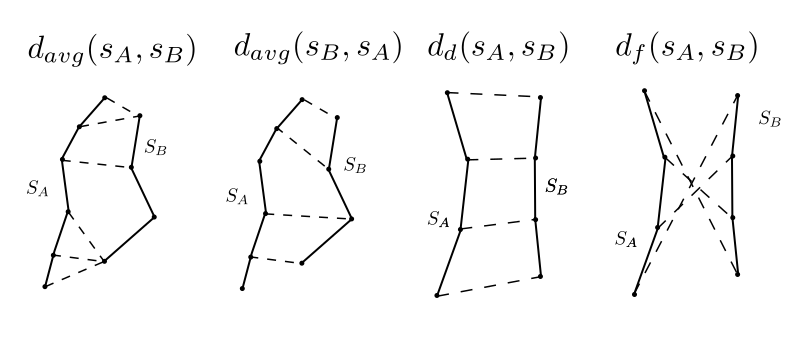
\includegraphics[scale=0.6]{distances}

\centering{}\label{Flo:Distances_used}\caption{Distances used in this work. The main distance used is minimum average
direct flip (MDF) distance $d_{\textrm{df}}=\min(d_{\textrm{d}},d_{\textrm{f}})$
which is a symmetric distance that can deal with the track bi-directionality
problem and works on tracks which have the same number of points.
Another distance is the mean average distance which is again symmetric
but does not need for the tracks to have the same number of points
$\textrm{MAM}_{\textrm{avg}}=(d_{avg}(s_{A},s_{B})+d_{avg}(s_{B},s_{A}))/2$.
In this figure the components of both distances are shown; with solid
lines we draw the tracks, and then with dashed lines we connect the
pairs of points of the two tracks whose distances contribute to the
overall metric.}

\end{figure}


Coming back to the MDF distance (see Eq.\ref{eq:direct_flip_distance}),
its main advantages are that it is fast to compute, it takes account
of track direction issues through consideration of both direct and
flipped tracks, and that it is easy to understand how it will behave,
from the simplest case of parallel equi-length tracks to the most
complicated with very divergent tracks. Another advantage is that
it will separate short tracks from long tracks and as we will see
this will be a good way to find broken or erroneous tracks. An advantage
of having tracks with the same number of points is that we can easily
do pairwise calculations on them; for example add two or more tracks
together to create a new average track . We will see in the next section
that track addition is a key property of our clustering algorithm.
Some care should be taken into consideration with the number of points
allowed in a track (track downsampling). We always keep the endpoints
intact and then downsample in equidistant segments. For example, short
tracks having the same number of points as long tracks means that
more of the curvature from the long tracks will be lost relative to
the short tracks i.e. the short tracks will have higher resolution.
We found empirically that this is not an important issue and that
for clustering purposes even downsampling to only $3$ points in total
could be useful \cite{EGMB10}. Depending on the application less
or more points can be used. 


\subsection{\label{sub:QB-Data-sets}Data sets}

This will be compressed into the Methods section.

We experimented with QuickBundles using simulations, $10$ human
tractographies collected and processed by ourselves and one tractography
with segmented bundles which was available online.

\textbf{Simulated trajectories.} We generated $3$ different bundles of
parametric paths samples at $200$ points. The tracks were made from
different combinations of sinusoidal and helicoidal functions.  In total
this data set contained $450$ tracks see Fig. \ref{Flo:simulated_orbits}.

\textbf{Human subjects. }We collected data from $10$ healthy subjects at
the MRC-CBU 3T scanner (TIM Trio, Siemens), using Siemens advanced
diffusion work-in-progress sequence, and STEAM
\cite{merboldt1992diffusion,MAB04} as the diffusion preparation
method. The field of view was $240\times240mm^{2}$, matrix size
$96\times96$, and slice thickness $2.5mm$ (no gap).  $55$ slices were
acquired to achieve full brain coverage, and the voxel resolution was
$2.5\times2.5\times2.5\textrm{mm}{}^{3}$. A $102$-point half grid
acquisition\cite{Yeh2010} with a maximum $b$-value of $4000\, s/mm^{2}$
was used. The total acquisition time was $14'21''$ with
TR=$8200\textrm{ms}$ and TE=$69\textrm{ms}$. The experiment was approved
by the local ethical committee CPREC.

For the reconstruction of the real data sets we used Generalized
Q-samping with diffusion sampling length $1.2$ and for the tractography
propagation we used EuDX (euler integration with trilinear
interpolation) with $1$ million random seeds, angular threshold
$60^{\circ}$, total weighting $0.5$, propagation step size $0.5$ and
anisotropy stopping threshold $0.0239$ (see
Fig. \ref{Flo:CloseToSelected},\ref{Flo:arcuate_close}).

\textbf{PBC human subjects}. We also used a few labeled data sets (see
Fig.\ref{Flo:cst_pbc},\ref{Flo:QB_fornix}), from the freely available
tractography database used in the Pittsburgh Brain Completion Fall
$2009$ ICDM pbc.lrdc.pitt.edu.

\subsection{Non-Metric Dissimilarities}

ROI-based connectivity matrix: \citep{ElKouby2005}

\section{QuickBundles (QB) Clustering}

\subsection{The QB Algorithm}

QuickBundles (QB) is a notably fast algorithm which can simplify
tractography representation in an accessible structure in a time that is
linear in the number of tracks $N$. QB is a linear time $O(N)$ (see
section \ref{sub:Complexity}) distance based clustering algorithm that
we created in order to clarify huge trajectory data sets such as those
produced by current state-of-the-art tractography generation algorithms
\cite{Parker2003,WWS+08}. In general, there are very few linear time
clustering algorithms. Just two are well known: CLARANS
\cite{ng2002clarans} and BIRCH \cite{zhang1997birch}. QB is different
from both of these methods; we will motivate it by describing some
aspects of BIRCH as a starting point for the presentation of QB.

BIRCH has two key components: first is relatively simple and involves
the use and updating of clusters' descriptors; second is the
construction of a tree structure in which the accumulated clusters are
held. This second component is aimed at maintaining efficient
searchability of the database while balancing what is kept in memory and
what is on disc for very large databases. BIRCH uses clustering
descriptors which are available for each item in the dataset; these are
specific vectors of a fixed dimension of numerical values. Each cluster
in turn has a descriptor which is an aggregate of the properties of the
items that belong to it (e.g. the sum or mean of the individual
clustering feature vectors). Proceeding by a single sweep through the
dataset, items are adjoined to clusters on the basis of their proximity
to the clusters, subject to a maximum cluster size, or they are added as
new leaves into the hierarchical tree structure in which the evolving
clusters are held. There then follow updating steps which can involve
the merging off previously created clusters in a k-means
fashion\cite{steinhaus1956division,macqueen1967some}.

It is the linear nature of BIRCH combined with the fixed dimensionality
of its cluster descriptors that makes it quite fast. However the further
steps involving reorganisation of the accumulated tree do add some major
overheads to BIRCH's performance. QB capitalises on these positive
features but does not try to create any kind of hierarchical structure
for the clusters. While items in BIRCH are fixed dimension vectors with
no additional structure, in QB each item (track) is a fixed-length
ordered sequence of points in $\mathbb{R}^{3}$, and uses metrics and
amalgamations which take account of and preserve this structure.
Moreover each item is either added to an existing cluster on the basis
of a distance between the cluster descriptor of the item and the
descriptors of the current set of clusters. Clusters are held in a list
which is extended according to need.

QB creates an online list of cluster nodes. The cluster node is defined
as $c=\{I,\mathbf{h},n\}$ where $I$ is the list of the integer indices
of the tracks in that cluster, $\mathbf{h}$ is an $p\times3$ matrix,
which the most important descriptor of the cluster, and $n$ is the
number of tracks on that cluster. $\mathbf{h}$ is a matrix which
can be updated online when a track is added to a cluster and is equal
to\begin{equation}
\mathbf{h}=\sum_{i=1}^{n}s_{i}\end{equation}
where $s_{i}$ is the $p\times3$ matrix representing track $i$,
$\Sigma$ here represents matrix addition, and $n$ is the number
of tracks in the cluster. QB assumes that all tracks have the same
number of points $p$, therefore a downsampling of tracks, typically
equidistant, is necessary before QB starts. A short summary of the
algorithm goes as follows. 

Select the first track $s_{0}$ and place it in the first cluster
$c_{0}\leftarrow\{0,s_{0},1\}$. Then for all remaining tracks (i)
goto next track $s_{i}$; (ii) calculate MDF distance between this
track and virtual tracks of all existing clusters $c_{k}$, where
a virtual track is defined on the fly as $\mathbf{v}=\mathbf{h}/n$;
(iii) if the minimum MDF distance is smaller than a distance threshold
$\mathrm{\mathit{thr}}$ add the track to the cluster $c_{j}=\{I,\mathbf{h},n\}$
with the minimum distance and update $c_{j}\leftarrow\{I\cup\{i\},\mathbf{h}+s,n+1\}$;
otherwise create a new cluster $c_{|C|+1}\leftarrow\{0,s_{i},1\}$,
$|C|\leftarrow|C|+1$ where $|C|$ denotes the current total number
of clusters. 

%
\begin{algorithm}
\textbf{Input} tracks $T=\{s_{0},...,s_{i},...,s_{|T|-1}\}$, threshold $\theta $\\
\textbf{Output} clustering $C=\{c_{0},...,c_{k},...,c_{|C|-1}\}$ where cluster $c=\{I,\mathbf{h},N\}$\\
\\
$c_{0}=\left\{0,s_{0},1\right\}$\\
$C=\left\{c_{0}\right\}$ \# the first track becomes the first cluster\\
$|C|=1$ \# the total number of clusters is 1 \\
$\textbf{For}$ $i$ $\textbf{From}$ $1$ $\textbf{To}$ $|T|-1$ $\textbf{Do}$ \# all tracks\\
\hspace*{2em} $\textbf{t}=T_{i}$\\
\hspace*{2em} $\texttt{alld}=\textbf{0}$ \# distance buffer\\
\hspace*{2em} $\texttt{flip}=\textbf{0}$ \# flipping check buffer\\
\hspace*{2em} $\textbf{For}$ $k$ $\textbf{From}$ $0$ $\textbf{To}$ $|C|-1$ \# all clusters\\
\hspace*{4em} $\mathbf{v}=C_{k}.\mathbf{h}/C_{k}.N$\\ 
\hspace*{4em} $d$=$d_{d}(\mathbf{t},\mathbf{v})$\\
\hspace*{4em} $f$=$d_{f}(\mathbf{t},\mathbf{v})$\\
\hspace*{4em} $\textbf{If}$ $f < d$ $\textbf{Then}$\\
\hspace*{6em} $d = f$\\
\hspace*{6em} $\texttt{flip}_{k} = 1$\\
\hspace*{4em} $\texttt{alld}_{k} = d$\\
$m=\min(\texttt{alld})$\\
$l=\mathrm{arg min}(\texttt{alld})$\\
$\textbf{If}$ $m < \theta$ \# append in current cluster \\
\hspace*{2em} $\textbf{If}$ $\texttt{flip}_{l}=1$ $\textbf{Then}$\\
\hspace*{4em} $C_{l}.\mathbf{h}+=t'$\\
\hspace*{2em} $\textbf{Else}$ \\
\hspace*{4em} $C_{l}.\mathbf{h}+=t$\\
\hspace*{2em} $C_{l}.N+=1$\\
\hspace*{2em} $C_{l}.I$.append($i$)\\
$\textbf{Else}$ \# create new cluster\\
\hspace*{2em} $|C|+=1$ \# total number of clusters increases\\
\hspace*{2em} $C_{|C|-1}.I_{0}=l$\\
\hspace*{2em} $C_{|C|-1}.\mathbf{h}=\mathbf{t}$\\
\hspace*{2em} $C_{|C|-1}.N=1$\\
\caption{QuickBundles}

\label{Alg:QuickBundles}
\end{algorithm}


Flipping can become an issue when using the MDF distance and adding
tracks together, because tracks do not have a preferred direction.
A step in QB takes account of the possibility of needing to perform
a flip of a track before adding it to a representative track. The
complete QB algorithm is described in detail in Alg.\ref{Alg:QuickBundles}
and a simple step by step visual example is given in Fig.\ref{Fig:LSC_simple}.
One of the reasons why QB has on average linear time complexity derives
from the structure of the cluster node: we only save the sum of current
tracks in the cluster and this is achieved cumulatively. By contrast
if we were using k-means at every iteration we would have to re-assign
tracks to clusters and recalculate averages which is computationally
much more intensive. Other reasons are that QB passes through the
tracks only once and that a track is assigned to one cluster only. 

QB is can be extended for specific applications to contain more information
about the clusters. For example we could redefine $c=\{I,\mathbf{h},n,\mathbf{h}^{(2)}\}$
to obtain second order information and in that way we could calculate
the variance of the cluster where \[
\mathbf{h}^{(2)}\leftarrow\{\sum_{i,j}x_{ij}^{2},\sum_{i,j}y_{ij}^{2},\sum_{i,j}z_{ij}^{2},\sum_{i,j}x_{ij}y_{ij},\sum_{i,j}y_{ij}z_{ij},\sum_{i,j}x_{ij}z_{ij}\}\]
 and $x_{ij},y_{ij},z_{ij}$ are the coordinates of the $j$th point
of the $i$th track in the cluster. Although this alternative would
be very useful, as even more refined cluster distances could be used
which take into account the additional information, this is not addressed
in this document.

%
\begin{figure}
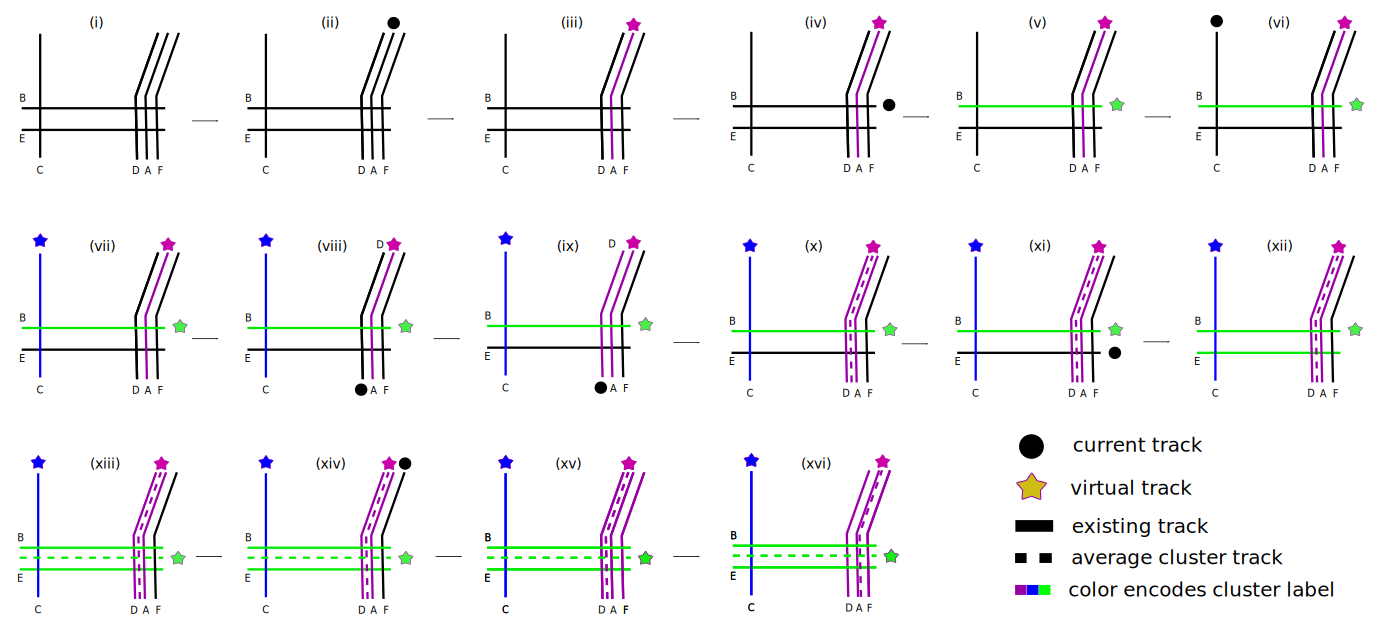
\includegraphics[scale=0.27]{last_figures/LSC_algorithm}

\label{Fig:LSC_simple}\caption{QB step-by-step: Initially in panel (i) 6 unclustered tracks (A-F)
are presented; imagine that the distance threshold used is the MDF
distance (Eq. [reference needed]) between B and E. The
algorithm starts and in (ii) we see that track A was selected, so
no other clusters exist therefore track A becomes the first cluster
(labeled with purple color) and the virtual track of that cluster
is identical with A as seen in (iii), next in (iv) track B is selected
and we calculate the MDF distance between B and the virtual track
of the other clusters. For the moment there is only one cluster to
compare so QB calculates MDF (B,virtual-purple) and this is obviously
bigger than threshold (that being MDF(B,E)) therefore a new cluster
is assigned for B and B becomes the virtual track of that cluster
as shown in (v). In (vi) the next track is selected and this is again
far away from both purple and blue virtuals therefore another cluster
is created and B is the virtual of the blue cluster as shown in (vii).
In (viii) track D is current and after we have calculated MDF(D,purple),
MDF(D,Blue) and MDF(D,green) it is obvious that D belongs to the purple
cluster as MDF(D,purple) is smaller and lower than threshold as shown
in (ix). However we can now see in (x) that things change for the
purple cluster because the virtual track is not anymore made by only
one track but it is the average of D and A shown with dashline. In
(xi) E is the current track and will be assigned at the green cluster
as shown in (xii) because MDF(E,virtual green) = MDF(E,B) = threshold,
and in (xiii) we see the updated virtual track for the green cluster
which is equal to (B+E)/2 where + means track addition. In (xiv) the
last track is picked and compared with the virtual tracks of the other
3 clusters; obviously MDF(F,purple) is the only with smaller threshold,
and so F is assigned to the purple cluster in (xv). Finally, in (xvi)
the virtual purple track is updated as (D+A+F)/3. As there are no
more tracks to select, the algorithm stops. We can see all three clusters
have been found and all tracks have been assigned successfully. }

\end{figure}

One of the disadvantages of most clustering algorithms is that they
give different results with different initial conditions; for example
this is recognised with k-means, expectation-maximization\cite{dempster1977maximum}
and k-centers\cite{gonzalez1985clustering} where it is common practice
to try a number of different random initial configurations. The same
holds for QB so if there are not distinct clusters such that the distance
between any pair of clusters is supra-threshold, then with different
permutations of the same tractography we will typically see similar
number of clusters but different underlying clusters. We will examine
the robustness of QB in this respect in section \ref{sub:Comparisons}.

subsection{Complexity and timings\label{sub:Complexity}}

To apply QB to a data set we need to specify three key parameters:
$p$, the fixed number of downsampled points per track; $\theta$
the distance threshold, which controls the heterogeneity of clusters;
and $N$ the size of the subset of the tractography on which the clustering
will be performed. When $\theta$ is higher, fewer more heterogeneous
clusters are assembled, and conversely when $\theta$ is low, more
clusters of greater homogeneity are created.

The complexity of QB is in the best case linear time $O(N)$ with
the number of tracks $N$ and worst case $O(N^{2})$ when every cluster
contains only one track. The average case is $O(MN)$ where $M$ is
the number of clusters however because $M$ is usually much smaller
than $N$ ($M\ll N$) we can neglect $M$ and denote it only as $O(N)$
as it is common in complexity theory. We created the following experiment
to investigate this claim and we found empirically that the average
case is actually $O(N)$ for tractographies (see Fig.\ref{Flo:Speed1},\ref{Flo:Speed2}).
In this experiment we timed the duration of QB clustering of tractographies
containing from $100$ thousand to $1$ million tracks, with different
initial number of points per track ($3,6,12$ and $18$) and different
QB thresholds ($10.0,15.0,20.0,25.00$ mm). The results can be seen
in the diagram of Fig.\ref{Flo:Speed1} and \ref{Flo:Speed2}. You
can notice that even when the the threshold value becomes impressively
low ($10.0$ mm) the linearity is only slightly disturbed.

%
\begin{figure}
\begin{centering}
\label{Flo:Speed1}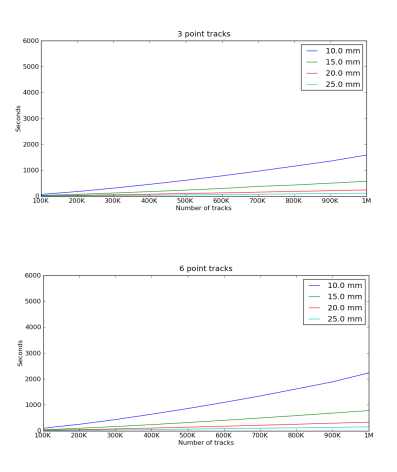
\includegraphics[scale=0.8]{last_figures/speed_3_6}
\par\end{centering}

\caption{QB is a very efficient algorithm whose performance is controlled by
just three parameters. The first is the number of tracks, a second
is the distance threshold in millimeters - shown with different colours
and another is the amount of initial downsampling of the initial trajectories.
A last parameter not shown in these diagrams is the underlying structure
of the data which is expressed by the number of final clusters. We
used a full tractography to generate these figures without removing
or preselecting any parts. This results run of a single thread Intel(R)
Xeon(R) CPU E5420 at 2.50GHz on a standard PC. (NB This and the following
figure use the same vertical scale to assist direct comparison.)}

\end{figure}

Furthermore, the memory usage of QB is $O(M)$ where $M$ is the number
of clusters and because this is usually much smaller than $N$ we
consider memory consumption to be negligible. Because in QB we store
only the indices of the tracks even for very large tractographies
$20$ or more clusterings can be stored simultaneously in the RAM
of a simple notebook without any problems. Therefore, another feature
of QB is memory efficiency.

%
\begin{figure}
\noindent \begin{centering}
\label{Flo:Speed2}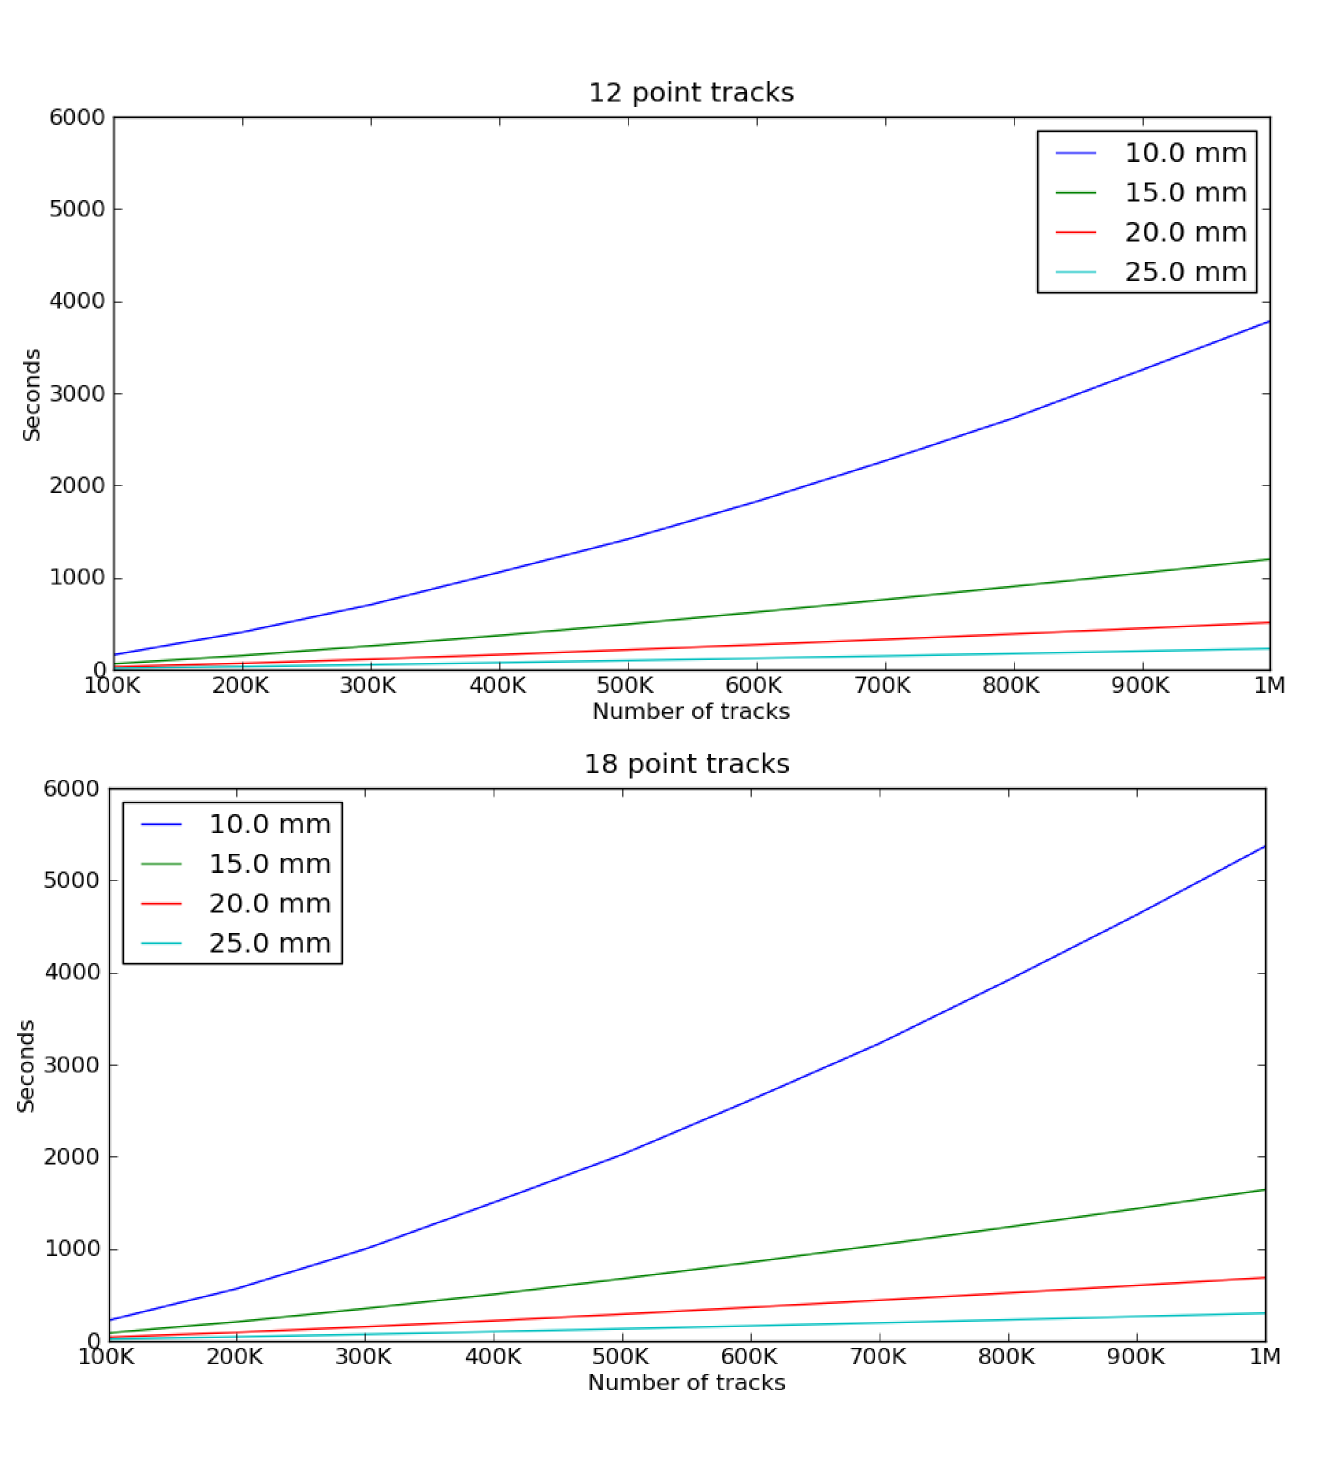
\includegraphics[scale=0.8]{last_figures/speed_12_18}
\par\end{centering}

\caption{Time comparisons of QB using different number of points per track,
different distance thresholds and different number of tracks. Same
as Fig. \ref{Flo:Speed1}. We can observe here how the linearity only
reduces slightly even when we use a very low threshold as that of
$10$mm which can generate many thousand clusters. This experiment
concludes that QB is suitable for fast clustering.}

\end{figure}

We compared QB with $12$ point tracks and distance threshold at
$\theta=10$mm versus some timings reported from other state of the art
methods found in the literature (Tab. \ref{Flo:timings}). Unfortunately
timings were very rarely reported up till now as most algorithms were
very slow on full data sets. Nonetheless the speedup that QB offers is
obviously of great importance and holds out the prospect of real-time
clustering on data sets of fewer than $20,000$ tracks (see
Tab. \ref{Flo:timings}).

%
\begin{table}
\small\addtolength{\tabcolsep}{-5pt}

\begin{centering}
\begin{tabular}{|c|c|c|c|c|}
\hline 
Number of tracks ($N$) & Algorithms & Timings (secs) & QB (secs) & Speedup\tabularnewline
\hline
\hline 
$1000$ & Wang et al. \cite{wang2010tractography} & $30$ & $0.07$ & $429$\tabularnewline
\hline 
$60,000$ & Wang et al. \cite{wang2010tractography} & $14400$ & $14.7$ & $980$\tabularnewline
\hline 
$400,000$ & Visser et al. \cite{Visser2010} & $75000$ & $160.1$ & $468$\tabularnewline
\hline
\end{tabular}
\par\end{centering}

\caption{QB run on $p=12$ point tracks and distance threshold at $\theta=10$mm
compared with some timings reported from other state of the art methods
found in the literature. Unfortunately timings were very rarely reported
until today as most algorithms were very slow on full data sets. Nonetheless,
we can observe in this table that the speedup that QB offers is substantial,
holding out the prospect of real-time clustering on data sets containing
fewer than $\sim20,000$ tracks. This experiment was executed on a
standard PC using only a single CPU core. }

\label{Flo:timings}
\end{table}

section{The QB Sketch}

One of the major benefits of applying QB to tractographies is that it
can provide meaningful simplifications and find structures that were
previously invisible or difficult to locate because of the high density
of the tractography. For example we used QB to cluster the corticospinal
tract (CST). This bundle was part of the datasets provided by the
Pittsburgh Brain Competition (PBC2009-ICDM) and it was selected by an
expert. The QB Sketch is clearly shown in Fig.\ref{Flo:cst_pbc} where
every cluster is represented by a single virtual track. To generate this
clustering we used a tight threshold of $10$mm. We observe that only a
few virtual tracks travel the full distance from bottom to top and that
they are many tracks that are broken (i.e. shorter than what was
initially expected) or highly divergent.

%
\begin{figure}
\begin{centering}
\label{Flo:cst_pbc}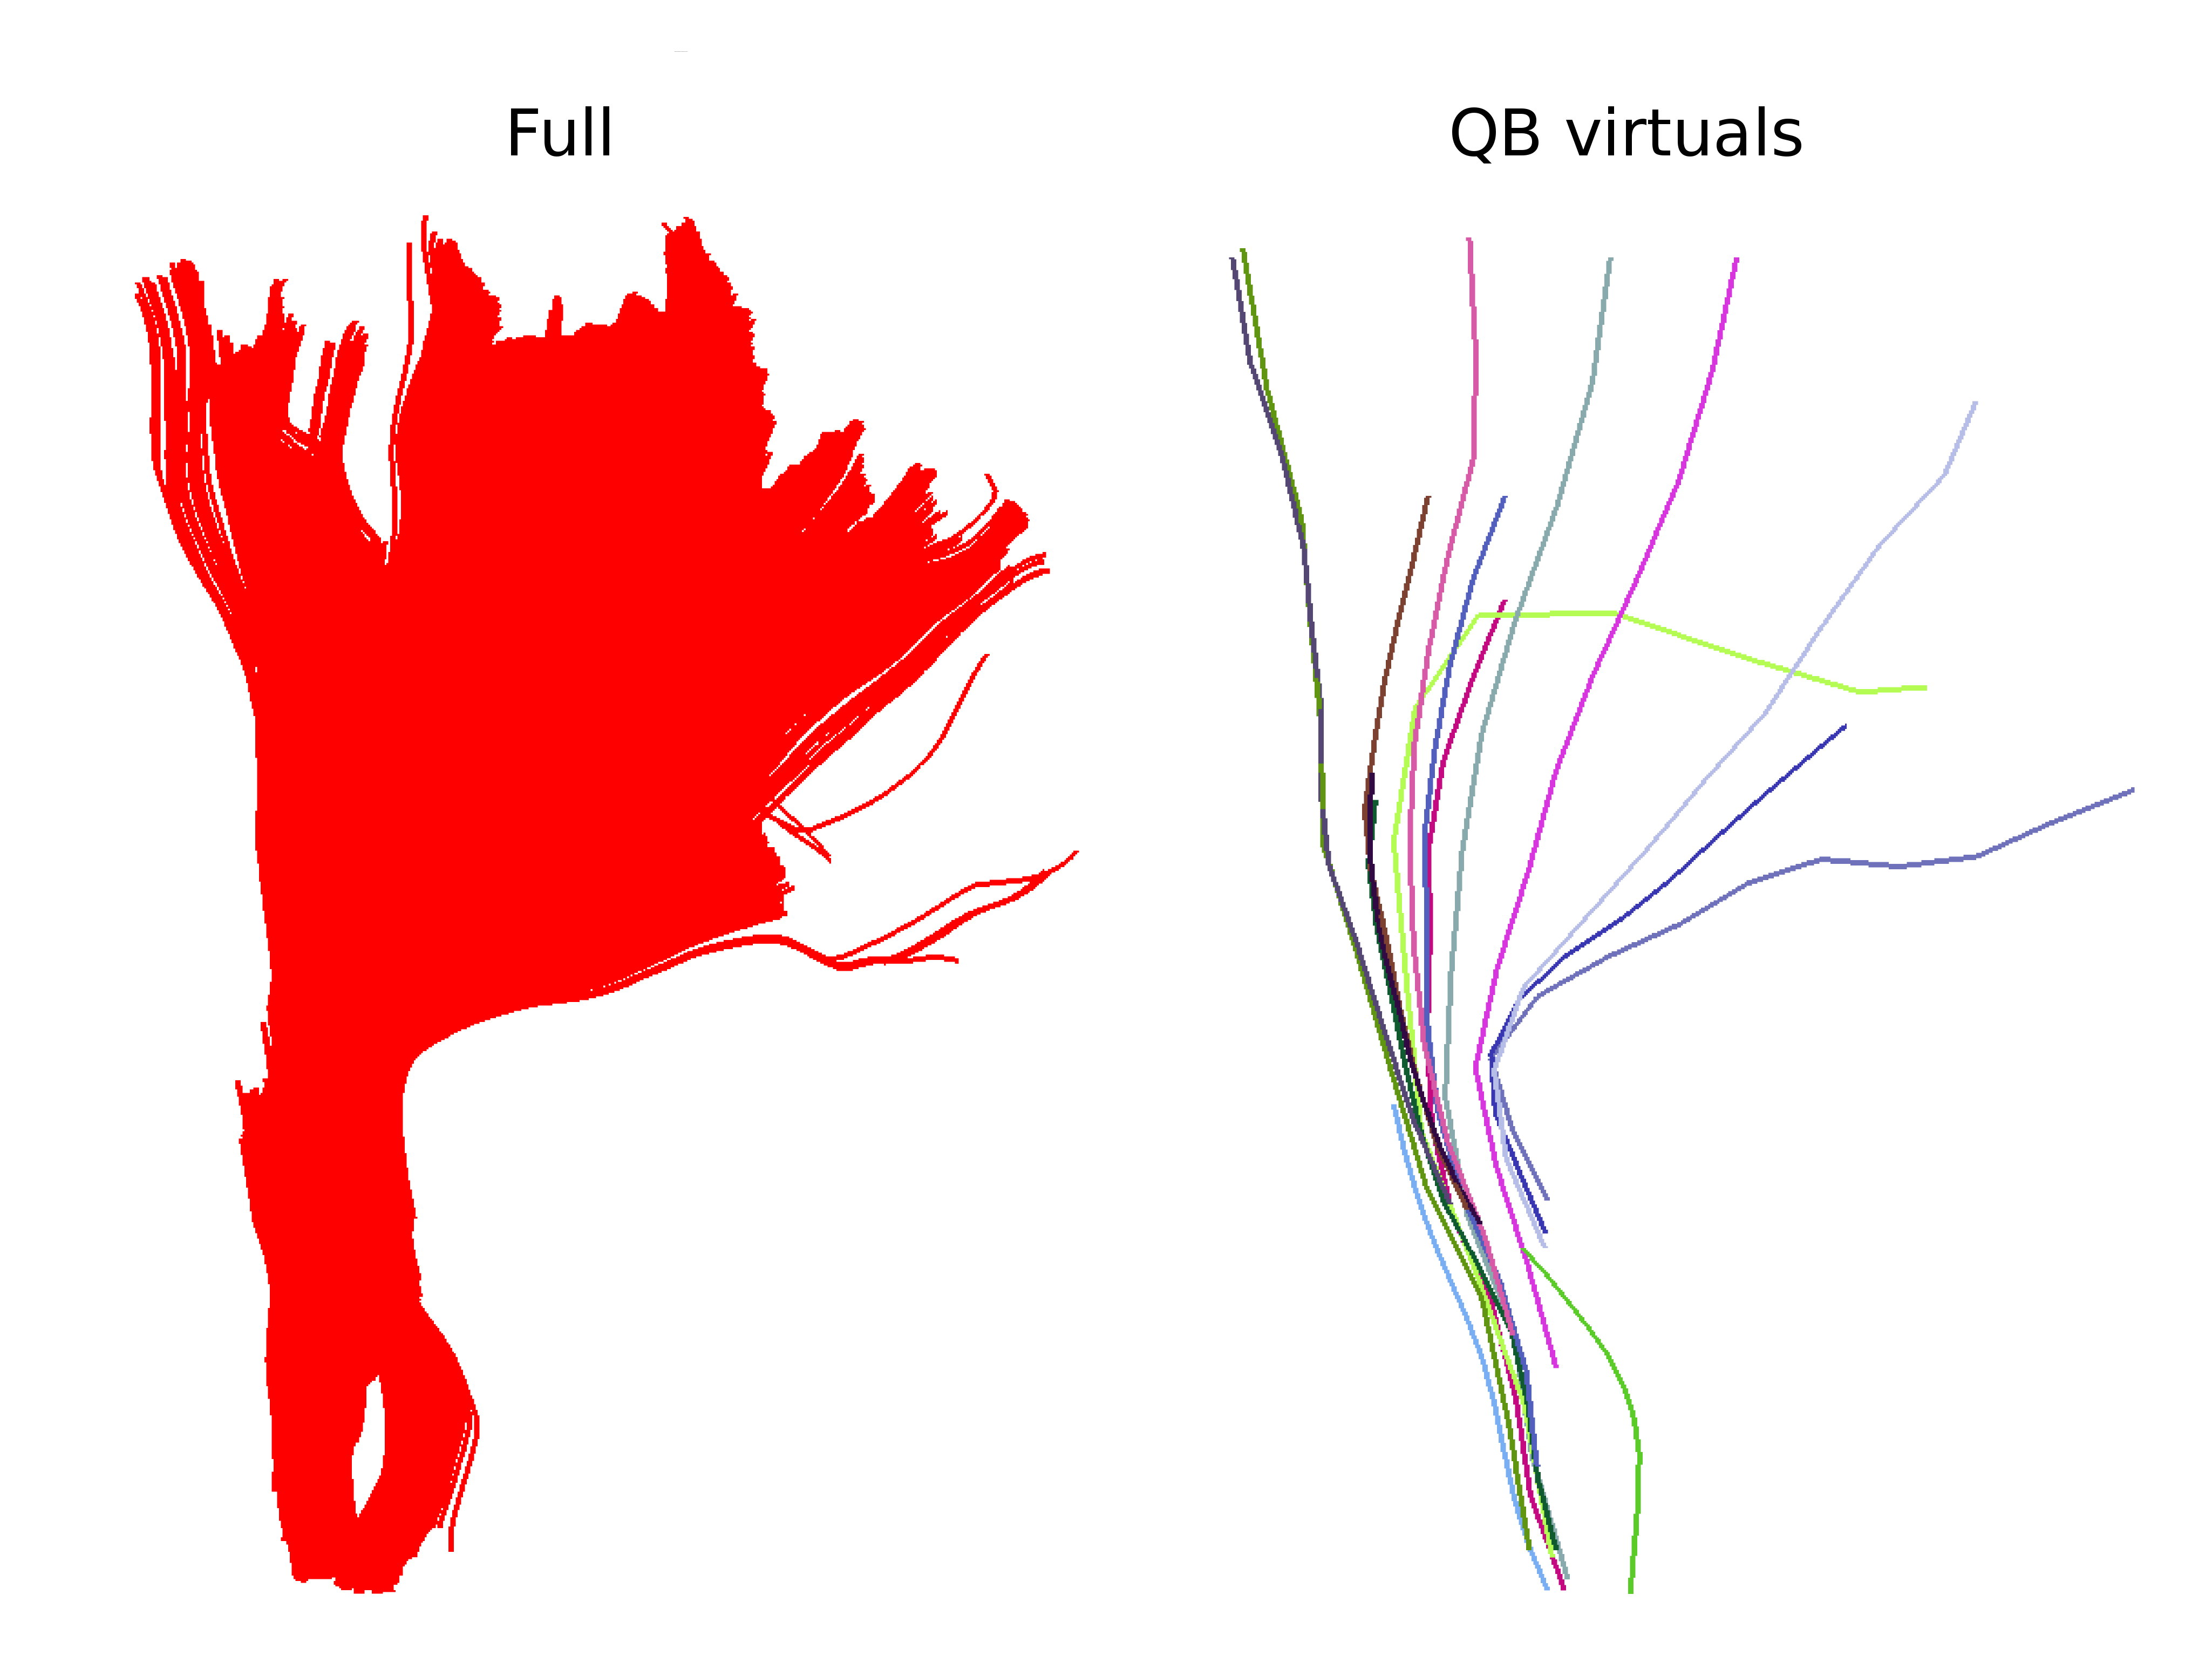
\includegraphics[scale=0.3]{last_figures/cst_simplification}
\par\end{centering}
\caption{This is a part of the CST bundle consisting of $11041$ tracks
  merged by an expert (PBC2009 data) shown with red color. Visually it
  looks as though all tracks have a similar shape, and possibly merge
  towards the bottom, and spreading towards the top. However, this is a
  misreading caused by the opaque density when all the tracks are
  visualised.  QB can help us see the full structure of the bundle and
  identify its elements. Here on the right hand side we see a
  simplification (virtual tracks) of the red CST generated by running QB
  with distance threshold of $10$ mm and downsampling to $12$ points. We
  can now clearly see that lots of parts which looked homogeneous are
  actually broken bundles e.g. dark green (A), light blue (C) or bundles
  with very different shape e.g. light green virtual track (B). To
  cluster this bundle took $135$ ms $\simeq$$0.14$ seconds.}

\end{figure}

Another interesting feature of QB is that it can be used to merge
or split different structures by changing the distance threshold.
This is shown in Fig. \ref{Flo:simulated_orbits}; on the left we
see simulated paths made from simple sinusoidal and helicoidal functions
packed together. The colour coding is used to distinguish the three
different structures. With a lower threshold the three different structures
keep remain separated but when we use a higher threshold the red and
blue bundles are represented by only one cluster; represented by a
purple virtual track.

%
\begin{figure}
\begin{centering}
\label{Flo:simulated_orbits}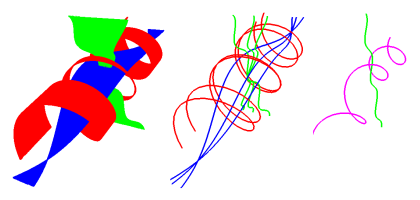
\includegraphics[scale=0.7]{last_figures/helix_phantom}
\par\end{centering}

\caption{On the left we see $3$ bundles of simulated trajectories; red,
  blue and green consisting of $150$ tracks each. All $450$ tracks are
  clustered together using QB and the virtual tracks are shown when
  threshold $1$ was used shown in the middle and $8$ on the right.  We
  can see that when the threshold is low enough the underlying structure
  is a more detailed representation of the underlying geometry. However
  when the distance threshold is higher closer bundles could merge
  together as seen in the result on the right panel where the red and
  blue bundle have merged together in one cluster represented by the
  purple virtual track.}

\end{figure}


Similarly, with the simulations shown in Fig.\ref{Flo:simulated_orbits}
we can see the same effect on real tracks, e.g. those of the fornix
shown at the left panel of Fig. \ref{Flo:QB_fornix} where we can obtain
different number of clusters at different thresholds. In that way we can
stress thinner or larger sub-bundles inside other bigger bundles.

%
\begin{figure}
\begin{centering}
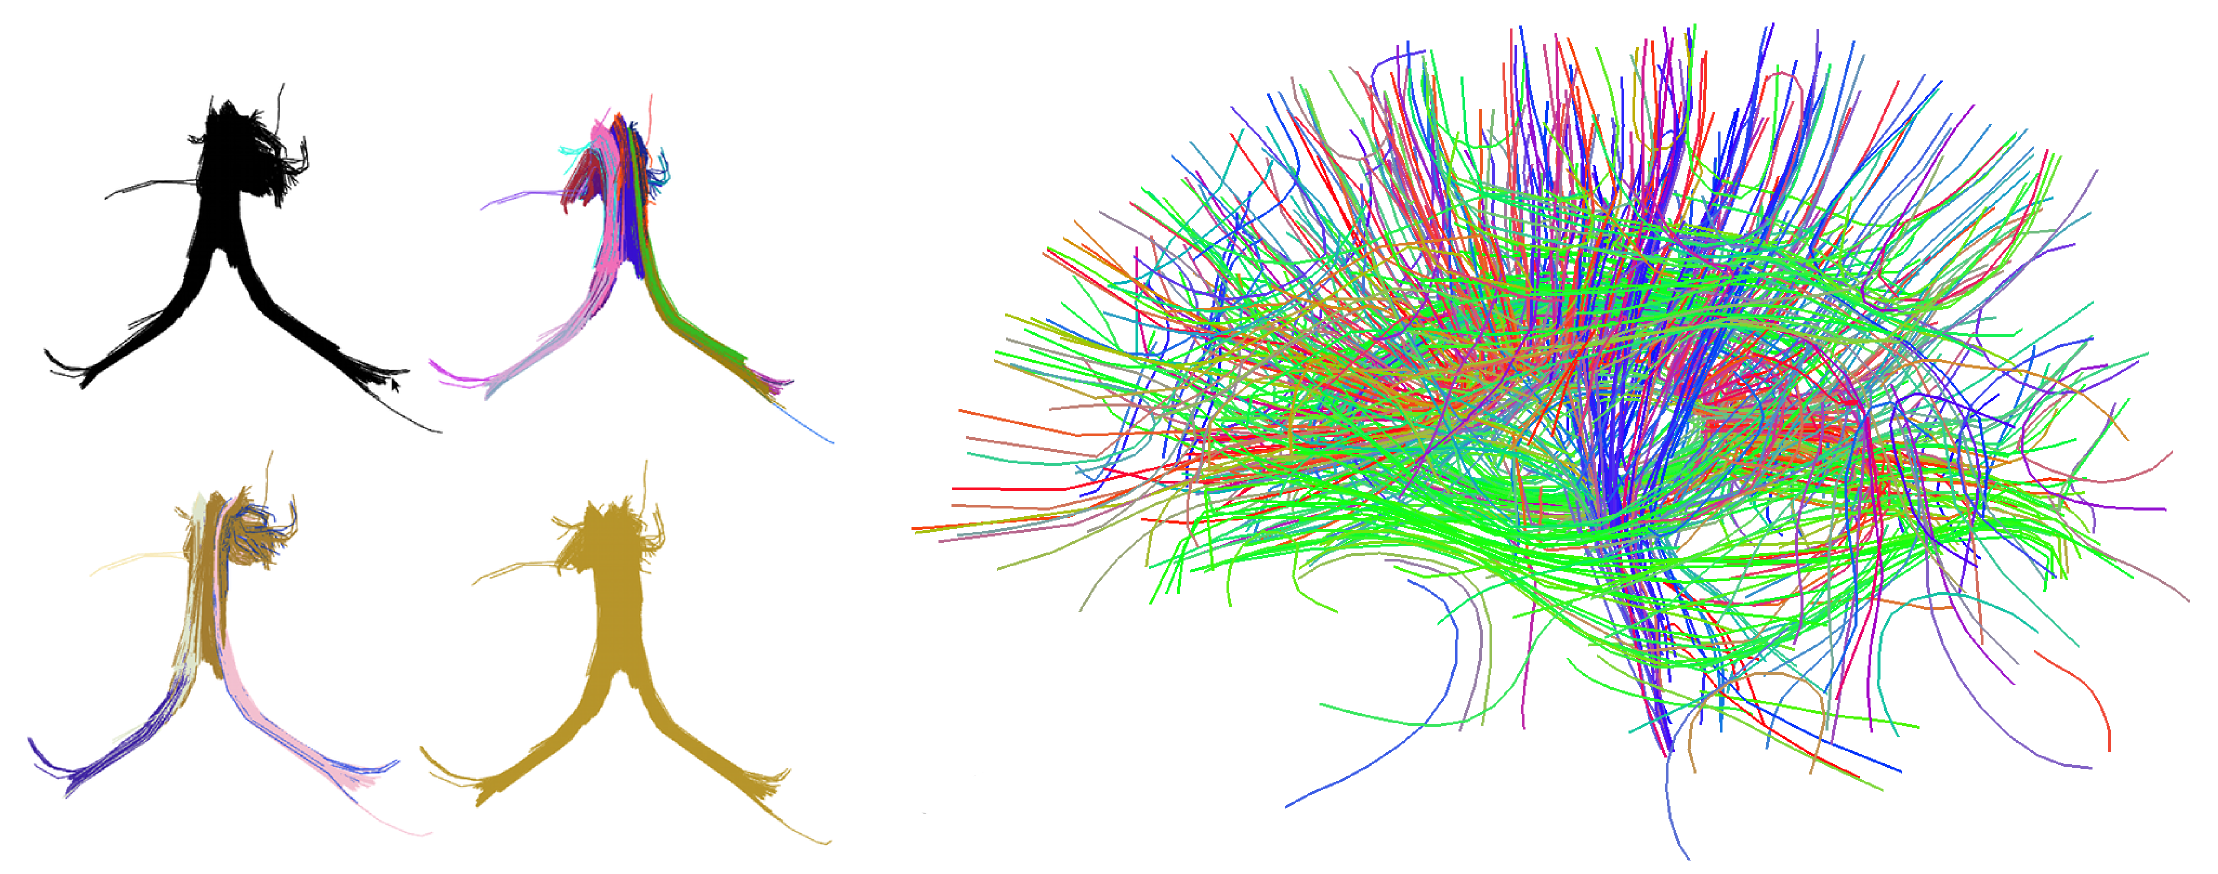
\includegraphics[scale=0.6]{last_figures/LSC_simple}
\par\end{centering}

\caption{Left - Here we see how QB clustered the fornix bundle with the
  dataset from the PBC2009 competition. The original fornix is shown in
  black consists of $1076$ tracks. All tracks were equidistantly
  downsampled at $3$ points in this example. With a $5$mm threshold our
  method generates $22$ clusters (top right). With $10$mm generates $7$
  (bottom left) and with $20$mm the whole fornix is determined by one
  cluster only (bottom right). Right - an example of a full tractography
  ($250,000$ tracks) being clustered using QB with a distance threshold
  of $10$mm. Here we see just $763$ virtual tracks depicted which
  produce a useful simplification of the initial tractography. Every
  track shown here represents an entire cluster from $10$ to $5000$
  tracks each. These can be thought as fast access points to explore the
  entire data set. The colour here just encodes track orientation.  With
  an appropriate visualization tool you could click on a track and
  obtain the entire cluster/bundle that it represents. Visualizing an
  entire data set of that size is impossible on standard graphic cards
  and most visualization tools e.g. Trackvis or DSI Studio can only show
  a small random sample of the full tractography at real time.}


\centering{}\label{Flo:QB_fornix}
\end{figure}


A full tractography containing $250,000$ tracks was clustered using QB
with a distance threshold of $10$mm (Fig. \ref{Flo:QB_fornix}).  We
produced a useful reduction of the initial tractography leaving only
$763$ virtual tracks. Bundles smaller than $10$ tracks were
removed. Every track shown here represents an entire cluster containing
from $10$ to $5000$ tracks each.

The virtual tracks can be thought as fast access points to explore the
entire data set (see Fig. \ref{Flo:QB_fornix}).


\subsection{Virtual tracks, exemplar tracks and other descriptors.}

The virtual tracks created by QB have very nice properties as they
represent an average track which can stand as the most important feature
of the cluster that they belong to. However, now that we have segmented
our tractography into small bundles we can calculate many more
potentially important descriptors for the cluster. For instance the
Cluster Spread (CS) can be computed for any cluster $c$ as a vector of
length $p$ whose $j$th component is $\sum_{x\in c}|x_{j}-v_{j}|^{2}/n.$
Here $x_{j}$ is the $j$-th point in the track $x$ in cluster $c$,
$v_{j}$ is the corresponding point of the virtual track, and $n$ is the
size of the cluster. CS provides a profile of the tightness or looseness
of the cluster along the length of the virtual track. Many other similar
or higher order statistics can be readily computed in an analogous
fashion. One of the most useful features is the calculation of
exemplars.

\textbf{Exemplars}. Another fruitful idea relating to the virtual track
is to try to identify a corresponding feature for the bundle which
actually belongs to the tractography. In other words to find an exemplar
or centroid track. Remember that the virtual tracks do necessarily
coincide with real tracks as they are just the outcome of large
amalgamations. There are many strategies for how to select good
exemplars for the bundles. A very fast procedure that we use in this
work is to find which real track from the cluster is closest (by MDF
distance) to the virtual track. Let's call this exemplar track $e_{1}$
such that $e_{1}={\displaystyle \argmin_{x\in C}}\textrm{\,\ MDF}(v,x)$.
The computational complexity of finding $e_{1}$ is still linear in
cluster size, and that will be very useful if we have created
clusterings with clusters containing more than $\sim5000$ tracks
(depending on system memory).

A different exemplar can be defined as the most similar track among all
tracks in the bundle, which we denote by $e_{2}={\displaystyle
  \argmin_{x\in C}}\,{\displaystyle \sum_{y\in C}}\mathrm{MDM(}y,x)$, or
if we want to work with tracks with possibly different numbers of points
we could instead use $e_{3}={\displaystyle \argmin_{x\in
    C}}\,{\displaystyle \sum_{y\in C}}\mathrm{MAM(}y,x)$.
Identification of exemplar tracks of type $e_{2}$ and $e_{3}$ will be
efficient only for small bundles of less than $5000$ tracks because we
need to calculate all pairwise distances in the bundle. We will see next
many applications of the exemplars. For example in the section
\ref{sub:The-bi-directionality-problem} we will use them to simplify the
bi-directionality problem when merging clusters.

In summary, a virtual (centroid) track is the average of all tracks in
the cluster. We call it virtual because it doesn't really exist in the
real data set and to distinguish it from exemplar (medoid) tracks which
are again descriptors of the cluster but are represented by real tracks.


\subsection{The bi-directionality problem\label{sub:The-bi-directionality-problem}}

Because a track is a sequence of points without a preferred direction,
it has two possible orientations when comparing it with another track.
Most tractography methods will create tracks with arbitrary directions;
meaning that close and similar tracks can have opposite directions.  Of
course the tracks do not really carry directional information.  By
direction we mean the encoding of the sequence of points which define
the track. Thus a track may be ordered $p_{1},p_{2}\ldots
p_{N-1},p_{N}$, or $p_{N},p_{N-1}\ldots p_{2},p_{1}$. We call this the
bi-directionality problem. Using the MDF distance we found a way with QB
to eliminate this problem. However, if we want to merge clusters
together we need to have a way to minimize this problem.

For this purpose we devised the following technique. Choose a fixed
point or pole $P$ in the 3D space of the tractography, possibly away
from the mid-sagittal plane. Then re-direct all tracks so that the first
point of every track is the end closer to $P$. If the tractography is in
native space it suffices to have the origin $(0,0,0)$ as the pole point;
in MNI space we can use the point $(100,100,100)$. It is our empirical
experience that this method will redirect correctly most tracks in the
sense that similar tracks will have the same direction.  However there
will still be a small percentage for which the bi-directionality problem
persists. We can correct for these by using exemplars rather than
virtual tracks as virtual tracks can misrepresent a bundle if the bundle
consists of tracks with ambiguous directionality. The exemplars are more
preferable than the virtual tracks because of the way the latter can be
influenced more by outliers and thus can be less representative in terms
of the shape of real tracks in a bundle. The exemplars are similar to
the concept of the median and the virtuals more similar to the concept
of the mean. It is well known that the mean is usually influenced more
by outliers than the median.

\section{\label{sub:Comparisons}Comparisons within- and between-subjects}

\subsection{Robustness under reordering}

As mentioned above, QB shares the behaviour of most clustering
algorithms in that different orderings of the tracks give rise to
different clusterings.  As a first step towards examining the robustness
of QB in this respect we recorded the numbers of QB clusters in $20$
different random orderings of the tractographies of $10$ human subjects
acquired as described in section \ref{sub:QB-Data-sets}. We removed
short tracks shorter than $40$mm and downsampled the tracks at $12$
points. Then we applied QB with threshold at $10$mm. The mean number of
clusters was $2645.9$ (min $1937.6$; max $3857.8$; s.d. $653.8$). There
is therefore a considerable between-subject variation in this metric. By
contrast the within-subject variability of the number of clusters across
random orderings is rather small, with mean standard deviation $12.7$
(min $7.3$; max $17.4$). This suggests an encouraging level of
robustness in terms of the numbers of clusters that QB creates. We now
consider ways of measuring and comparing the contents of the clusters in
a clustering.


\subsection{Tightness comparisons\label{sub:Tightness-comparisons-1}}

We have found rather few systematic ways to compare different clustering
results for tractographies in the literature\textbf{
}\cite{moberts2005evaluation}.  Being able to compare results of
clusterings is crucial for creating stable brain imaging procedures, and
therefore it is necessary to develop a way to compare different
clusterings of the same subject or different subjects. Although we
recognise that this is a difficult problem, we propose the following
solution with a metric which we call tight comparison (TC). Tight
comparison works as follows. Let us assume that we have gathered the
exemplar tracks from clustering $A$ in $E_{A}=\{e_{1},...,e_{|E_{A}|}\}$
and from clustering $B$ in $E_{B}=\{e_{1}^{'},...,e_{|E_{B}|}^{'}\}$
where $|E|$ denotes the number of exemplar tracks of each clustering
$E$. The size of set $E_{A}$ does not need to be the same as that of
$E_{B}$ (i.e.  perhaps $|E_{A}|\neq|E_{B}|$ rather then
$|E_{A}|=|E_{B}|$). Next, we calculate all pairwise MDF distances
between the two sets and store them in rectangular matrix $D_{AB}$. The
mimima of the rows of $D_{AB}$ provide the distance to the nearest track
in ${\cal B}$ of each track in $A$ ($E_{A\rightarrow B}$) and similarly
the minima of the columns of $D_{AB}$ the distance to the nearest track
in $A$ of each track in $B$ ($E_{B\rightarrow A}$). From these
correspondences we only keep those distances that are smaller than a
tight (small) threshold $t_{t\textrm{hr}}$. Then we define TC (Tightness
Comparison) to be

\begin{equation}
TC=\frac{1}{2}\left(\frac{|E_{A\rightarrow B}\leq t_{\textrm{thr}}|}{|E_{A}|}+\frac{|E_{B\rightarrow A}\leq t_{\textrm{thr}}|}{|E_{B}|}\right)\end{equation}


where $|E_{A\rightarrow B}\leq t_{\textrm{thr}}|$ denotes the number of
exemplars from A which had a neighbour in B that is closer than
$t_{\textrm{thr}}$ and similarly for $|E_{B\rightarrow A}\leq
t_{\textrm{thr}}|$ the number of exemplars from B to A which their
distance was smaller than $t_{\textrm{thr}}$. When $TC=0$ that means
that every exemplar from the one set was further than $t_{\textrm{thr}}$
to all exemplars in the other set. When $TC=1$ then all exemplars from
one set had a close neighbour in the other set. This metric is extremely
useful especially when comparing tractographies from different subjects
because it does not require $|E_{A}|=|E_{B}|$.

We ran an experiment were we compared TC between pairs of $10$ subjects
with their tractographies warped in MNI space. This generated
$\binom{10}{2}=45$ TC values with $t_{\textrm{thr}}=$$10$mm. We did this
experiment twice; first by keeping only the bundles with more than $10$
tracks (TC10) and secondly by keeping only the bundles with more than
$100$ tracks (TC100). The average value for TC10 was $47\%$ and standard
deviation $2.6\%$. As expected TC100 (bigger landmarks) did better with
average value of $53\%$ and standard deviation $4.9\%$. The difference
between TC10 and TC100 is highly significant: Student's t$=4.692$,
df=88, $p=1.97\times10^{-5}$, two-sided; and, as a precaution against
non-normality of the underlying distributions, Mann-Whitney U = 530.,
$p=5.65\times10^{-5}$. If we think that the small bundles of size $<100$
are more idiosyncratic or possibly more likely to reflect noise in the
data, whereas larger bundles are more indicative of substantial
structures and landmarks in the tractographies, then we are encouraged
to see that on average the virtual tracks of $50\%$ of larger bundles of
each tractography lie within$10$mm of those of the other
tractographies. This supports the notion that QB can be used to find
agreements between different brains by concentrating on the larger (more
important) clusters. We will see further evidence for this below
(section \ref{sub:Atlases-made-easy}).


\subsection{Merging two sets of bundles}

We can merge bundles using exemplar tracks or virtual tracks. We first
set a distance threshold $\theta$ usually the same as the one we used
for the QBs in the previous step. Let's assume now that we have gathered
the virtual tracks from clustering $A$ in
$V_{A}=\{v_{0},...,v_{|V_{A}|}\}$ and from clustering $B$
in$V_{B}=\{v_{0}^{'},...,v_{|V_{B}|}^{'}\}$ where $|V|$ denotes the
number of virtual tracks of each clustering.  $|V_{A}|$ can be different
$|V_{B}|$. (a) For every $v_{i}^{'}$ in set $V_{B}$ we find the closest
$v_{j}$ in set $V_{A}$ and store the distance between these two
tracks. Therefore we now have a set of minimum distances from $V_{B}$ to
$V_{A}$. The size of this set is equal to $|V_{B}|$. (b) Finally, we
merge those clusters from $B$ whose virtual tracks have minimum
distances smaller than $\theta$ into the corresponding clusters of $A$,
and if a virtual track in $V_{B}$ has no sub-threshold neighbour in
$V_{A}$ then its cluster becomes a new cluster in the merged
clustering. In that way clusters from the two sets who have very similar
features will merge together and if not new clusters will be created,
and we will not have any loss of information from the two sets of
clusters.


\section{Parallel version\label{sub:Parallel-version}}


\subsection{Algorithm}

QB is a very fast algorithm; however we wanted to make it even more
efficient so that for example it is trivial to cluster hundreds of
subjects together and use many CPUs or computers simultaneously. This
could be used to create an atlas of hundreds of subjects in a few
hours. Therefore, we have extended QB to a parallel version which we
call pQB. This algorithm works as follows. First we redirect and
downsample all tracks. Then we put all tracks together and break them
into subsets. For every subset we assign a new thread and set QB to run
on that thread. Therefore, we have now many QBs running on different
CPUs. Then we collect all individual clusterings and start merging them
together. We can pair every two results together and merge them in a
binary way or just merge all clusterings to the first clustering.  We
can do merging with many different ways. Here we present the most modest
but useful attempt.

\section{Direct applications}

We found that QB has numerous applications from detecting erroneous
tracks to creating atlases, finding landmarks and guiding registration
algorithms. Here we present just a few of the strategies that can be
pursued further.


\subsection{Rapidly detecting erroneous tracks}

It is well known that there are different artifacts seen in
tractographies caused by subject motion, poor voxel reconstruction,
incorrect tracking and many other reasons. However there is no known
automatic method to try and detect these tracks and therefore remove
them from the data sets. The idea here is to use QB to speed up the
search for erroneous tracks. We will concentrate here on tracks that
loop one or many times; something that it is considered impossible to
happen in nature.

One of the tracks which are most likely erroneous are tracks which wind
more than one time, like a spiral. We can detect those with the
following algorithm. Lets assume that we have a track $s$ and we want to
check if it winds: (a) we perform a singular value decomposition on the
centered track $U,\mathbf{d},V=\mathtt{SVD}(s-\bar{s})$; (b) project the
highest singular value $\mathbf{d_{0}}$ to the first column of $U,$
$U_{o}$ creating the first component of a two dimensional coordinate
$p_{x}$ and the second highest $\mathbf{d_{1}}$ to the second column
$U_{1}$ creating the second coordinate $p_{y}$; and (c) calculate the
cumulative winding angle on the 2d plane; d) if the cumulative angle is
more that $400^{\circ}$ then that would mean that the initial track $s$
is winding and therefore needs to be removed, see
Fig. \ref{Flo:winding}.

Winding tracks can be dangerous when we merge clusters because they
could be close to many different clusters. We found that winding tracks
often form bundles with many similar tracks. Also, they are usually long
tracks so they will not be removed with any filters which remove short
tracks. We could use QB with a low threshold to reduce the number of
tracks while avoiding embedding winding tracks into otherwise ordinary
clusters and then run the winding algorithm just on the exemplar tracks
of the bundles rather than the entire tractography.

%
\begin{figure}
\begin{centering}
\label{Flo:winding}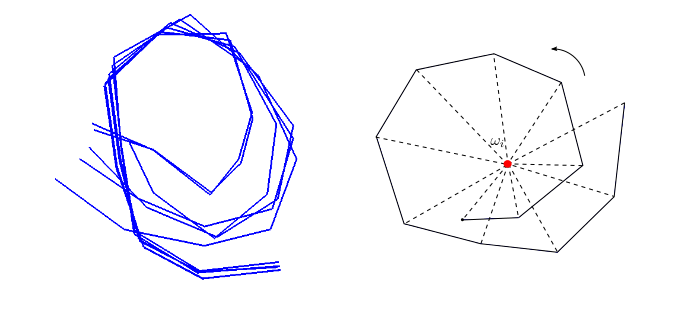
\includegraphics[scale=0.5]{last_figures/winding}
\par\end{centering}

\caption{Example of detecting a possibly erroneous 3D bundle (on the
  left) by projecting its exemplar track and counting the winding
  cumulative angle $\sum_{0}^{N}\omega_{i}$ on the 2D plane as shown on
  the right, where $N$ is the total number of track segments. Usually
  bundles with total angle higher than $400^{\circ}$ are removed from
  the data sets as most likely to be erroneous.}

\end{figure}


QB can also simplify detection of tracks which are very dissimilar to
others and therefore they are very distant from all other clusters.
Usually when we use a QB threshold of about $10$mm these tracks will be
part of small bundles containing a few tracks ($<10$) and the distance
of the bundle they belong to from all other bundles will be much higher
than average. This can give us another detection method for outliers.

Finally, QB can be used to remove small or broken tracks in an
interactive way, for example see Fig. \ref{Flo:cst_pbc} where the red
large bundle has been merged by an expert and then with QB we can
extract the skeleton of the bundle and see which parts create that
structure. Without QB it would be too difficult to work out that this
bundle consists of many small or divergent parts. In this figure both
very diverging, small or broken tracks can be identified after the
simplification provided by QB.

In summary, we have shown that QB can facilitate a fully automatic,
efficient and robust detection system for erroneous tracks in specific
bundles or entire tractographies.

%
\begin{figure}
\begin{centering}
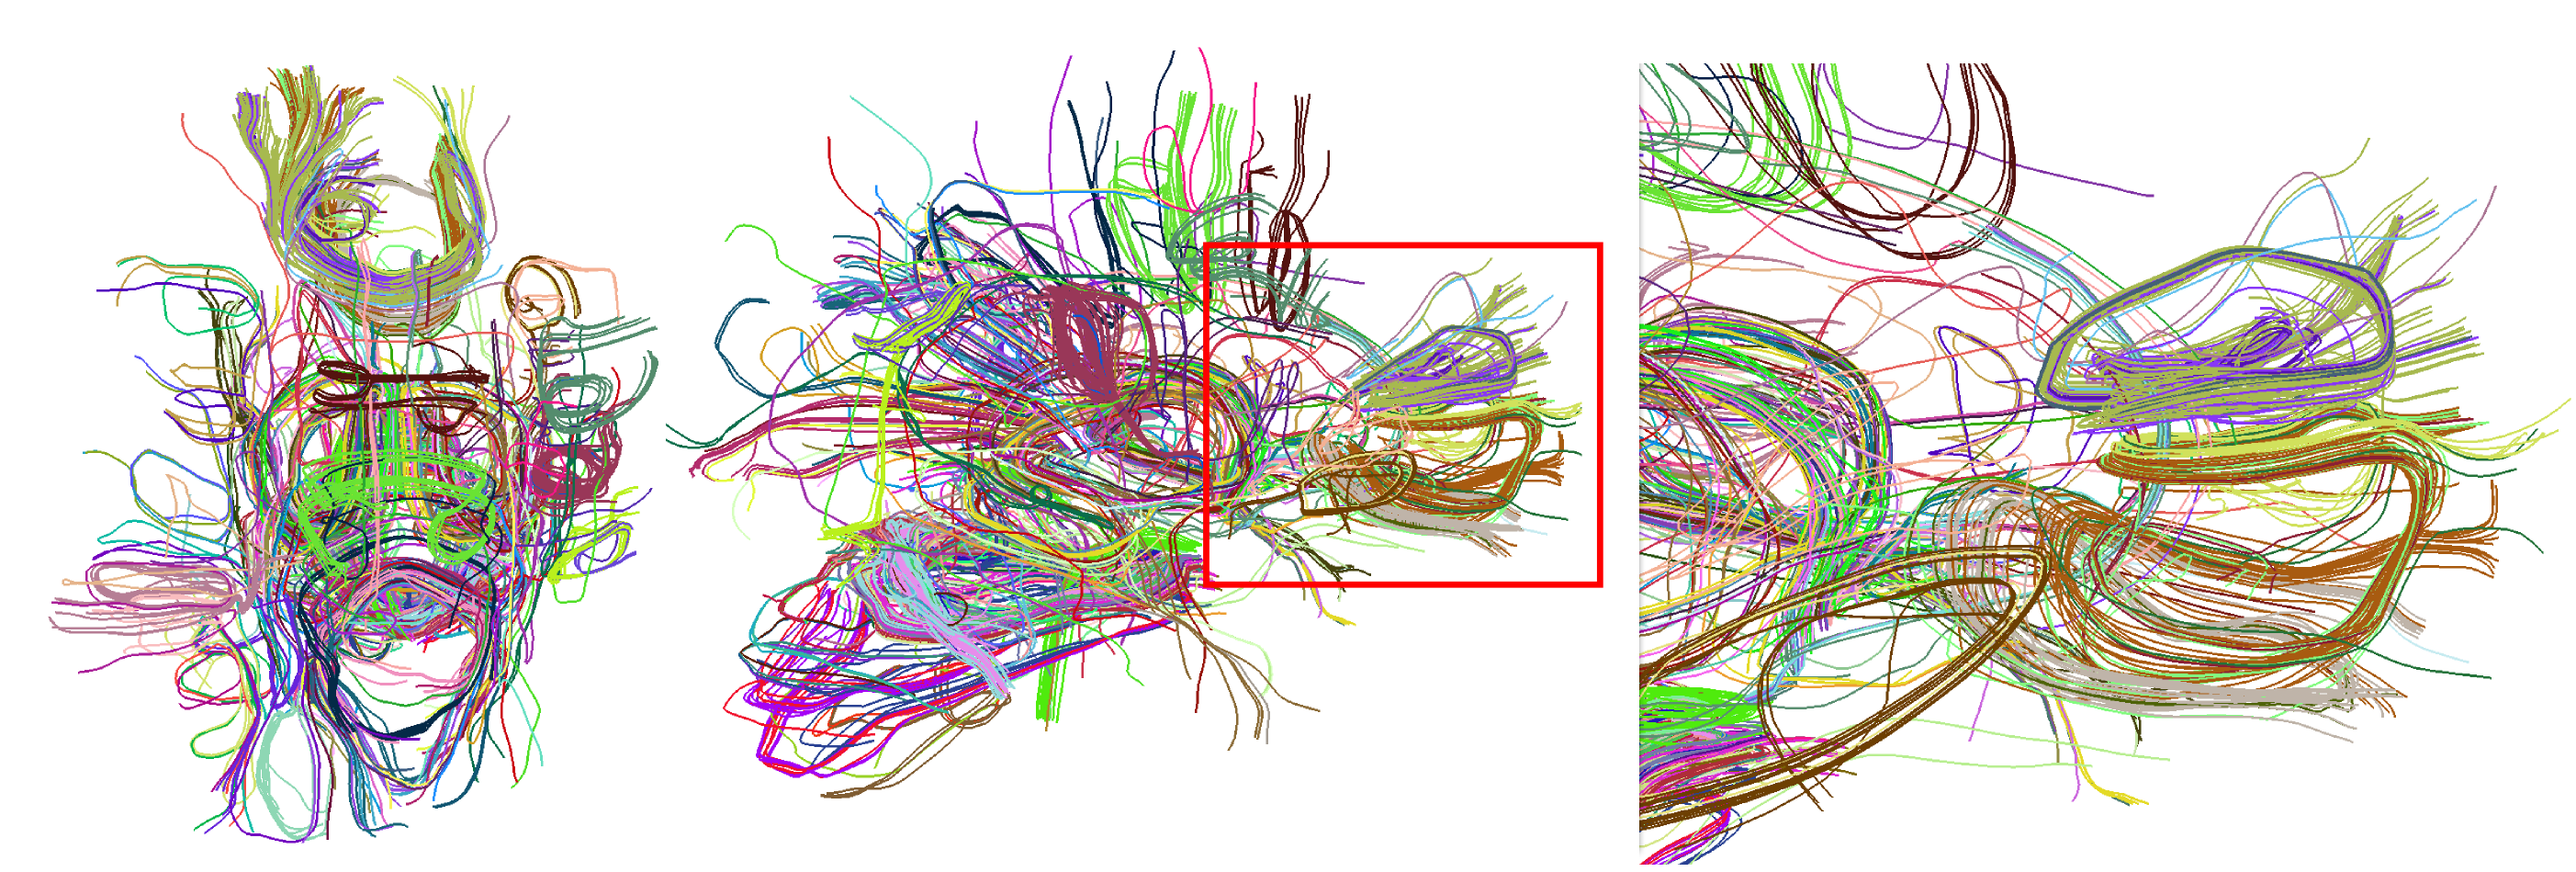
\includegraphics[scale=0.65]{last_figures/erroneous_tracks}
\par\end{centering}

\label{Flo:erroneous_tracks}
\caption{$161$ most likely erroneous bundles automatically detected by
  our winding method all having total winding angle higher than $500$
  degrees and shown with random colours per bundle. On the left panel we
  see the bundles on their exact position in the data set from the top
  of the head, on the middle panel we see the same tractography from the
  side and the third panel we see the part of middle panel on the red
  box slightly rotated and much zoomed so that some erroneous tracks can
  be easily shown. To cluster the initial tractography not shown here we
  used QB with threshold $10$mm. This is the first known automatic
  detection system of outliers and erroneous tracks for tractography
  data based on more advanced shape characteristics that go beyond
  simple length. By calculating the number of winding tracks in your
  data sets over the total number of tracks you can have an indicator of
  the quality of our data sets.}

\end{figure}



\subsection{Alignments, landmarks and atlases\label{sub:Atlases-made-easy}}

We have used QB to construct a robust tractographic atlas in MNI space
from data for 10 subjects. Here we explain the steps we used to achieve
that.

\textbf{Alignment}. Tractographies were created using EuDX as described
in section \ref{sub:QB-Data-sets} and see section
[reference needed] for acquisition details. The
tractographies for all subjects were initially in native space and the
goal was to warp them in MNI space, using nonlinear registration.

Because the registration of tractographies is generally considered a
difficult problem with a non-unique solution we wanted to make sure that
we are using a known, well established and robust method, therefore we
chose to use $\texttt{fnirt}$ with the same parameters as used with the
first steps of TBSS\cite{Smith2006NeuroImage}. For that reason FA
volumes were generated from the same data sets using Tensor fitting with
weighted least squares after skull stripping with $\texttt{bet}$ and
parameters $\texttt{-F -f .2 -g 0}$. These FA volumes were again in
native space therefore we needed to warp them in MNI space. For this
purpose a standard template ($\texttt{FMRIB58\_FA\_1mm}$) from the FSL
toolbox was used as the reference volume. However, we wanted primarily
to have the displacements which would do a point wise mapping from
native space to MNI space and we found this to be technically very
difficult with the FSL tools as they assume that these displacements
will be applied only on volumetric data and not with point data as those
used in tractographies. Finally, after some considerable effort we found
a combination of $\texttt{flirt}$, $\texttt{invwarp}$,
$\texttt{fnirtfileutils}$ and $\texttt{fnirtfileutils -withaff}$ which
gave us the correct displacements. As this being very technical we will
not describe it further here but the code is available in module
($\texttt{dipy.external.fsl}$). It is also important to say that we
didn't use eddy correction with any of this type of data sets because
eddy correction is unstable with volumes at high b-values because there
is no much signal for guiding a correct registration with the other
volumes at lower b-values.

After creating the displacements for every subject; these were applied
to all tractographies in the native space so they are mapped in the MNI
space of voxel size $1\times1\times1\textrm{mm}^{3}$. Having all
tractographies in MNI space is something very useful because we can now
compare them against available templates or against each other and
calculate different statistics. However this is not where we stop; we
proceed to generate a tractographic atlas using QB clusterings.

\textbf{Tractographic Atlas.} For all subjects, (a) load warped
tractography (b) re-direct towards a static point $(100,100,100)$ as
explained in section \ref{sub:The-bi-directionality-problem}, (c)
downsample the tracks to have only $12$ points, (d) calculate and store
QB clustering with a $10$mm threshold. Then merge all clusterings again
with $10$mm threshold as explained in section \ref{sub:Parallel-version}
(merging).  When creating an atlas by merging many different subjects
the most important issue is what you remove from the atlas as
outliers. QB here provides a possible solution for this problem. If we
plot the number of tracks for each cluster sorted in ascending order we
can see an interesting pattern see Fig.\ref{Flo:atlas_big_bundles}. In
this diagram we observe that $20\%$ of the largest clusters had more
than $90\%$ of the total amount of tracks. This shows that there is much
agreement between the biggest bundles of different subjects.  We will
use this property to create a solid atlas in which we keep the biggest
bundles (landmarks) and remove small bundles (outliers).

%
\begin{figure}
\centering{}
\label{Flo:atlas_big_bundles}
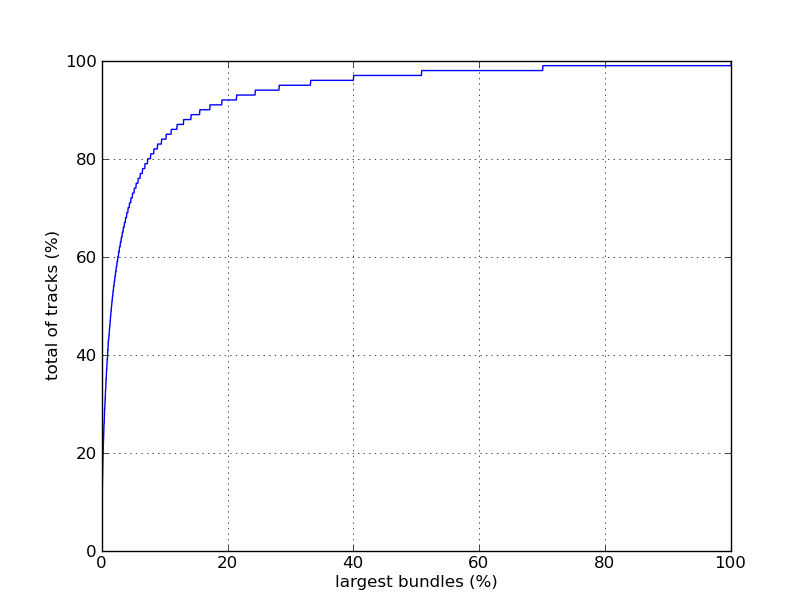
\includegraphics[scale=0.6]{last_figures/big_bundles_atlas}
\caption{$14520$ clusters where created by joining the QB clusterings of
  $10$ subjects in MNI space. We found that most of the clusters had a
  few tracks and only a few clusters had many. In the diagram above we
  can see $20\%$ of the largest clusters had more than $90\%$ of the
  total amount of tracks. This result showed that there is much
  agreement between different subjects which would be useful for a solid
  atlas with the biggest bundles becoming landmark bundles and the small
  bundles removed as outliers.}

\end{figure}

\textbf{Finding and Using Landmarks}

One can use this atlas or similar atlases created from more subjects in
order to select specific structures and study these structures directly
in different subjects without using any of the standard ROI based
methods.

A simple example is given in Fig. \ref{Flo:CloseToSelected}. In the
first row we see a tractographic atlas joined by merging the QB
clusterings of $10$ healthy subjects as described in the previous
section. Then from these clusters represented by their virtual tracks we
keep only $196$ biggest clusters i.e. those which contain the highest
number of tracks, so that we are sure that there is enough agreement
from the different tractographies and from these we just pick by way of
an example $19$ virtual tracks which correspond to well known bundle
structures in the literature: $1$ from genu of corpus callosum (GCC),
$3$ from the body of corpus callosum (BCC), $1$ from the splenium (SCC),
$1$ from the pons cerebellar peduncle (CP), $1$ from left arcuate
fasciculus (ARC-L), $1$ from right arcuate fasciculus (ARC-R), $1$ from
left inferior occipitofrontal fasciculus (IFO-L) and $1$ from right
inferior occipitofrontal fasciculus (IFO-R), $1$ from right fornix
(FX-R), $1$ from left fornix (FX-L), $1$ optic radiation (OR), $1$ left
cingulum (CGC-L), $1$ from right cingulum (CGC-R), $1$ from left
corticospinal tract (CST-L), $1$ from right corticospinal tract (CST-R),
$1$ from left uncinate (UNC-L) and $1$ from right uncinate
(UNC-R). These $19$ tracks are coloured randomly. Then on the second row
we show, for the first $6$ of these selected representative tracks, the
tracks closer than $20$mm from $3$ arbitrarily selected
subjects. Similarly, on the third row the tracks closer than $15$mm to
the next $7$ selected tracks. Finally on the last row we bring the
tracks from the same $3$ subjects which are closer than $18$mm.  The
colours used for the selected tracks are automatically assigned from the
colours of tracks picked from the atlas. We can see that there is a
significant reliability and continuity both within and between subjects
even though we have only selected a very small number of representative
tracks. Using a similar procedure we could create a book of bundles for
every subject and then compare the subjects at the level of bundles.

%
\begin{figure}
\begin{centering}
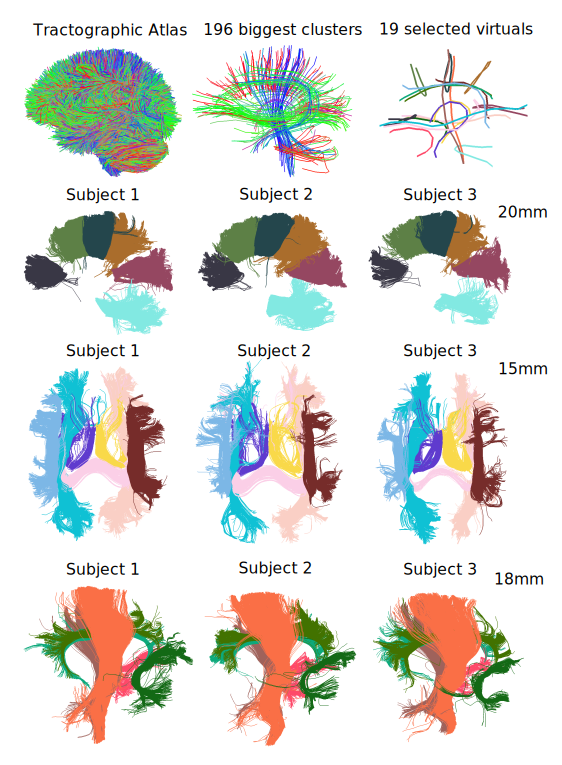
\includegraphics[scale=0.7]{last_figures/close_distance}
\par\end{centering}

\label{Flo:CloseToSelected}
\caption{A novel way to do comparisons between subjects. Correspondence
  between different subjects (last $3$ rows) and a few landmarks picked
  from the tractographic atlas generated by merging QB clusterings of
  $10$ subjects (top row). That we can see this amount of agreement and
  continuity on the last $3$ rows from such a few skeletal tracks is a
  great hope for implementing new robust ways of statistical comparisons
  using tractographic data sets.}

\end{figure}

\subsection{QB as input to other learning methods}

We found that QB is of great value as an adjunct to many less efficient
algorithms e.g. hierarchical clustering, affinity propagation, nearest
neighbours, spectral clustering and other unsupervised and supervised
learning methods. We present here one example with QB as input to
affinity propagation and one with QB as input to hierarchical
clustering.

Most clustering algorithms need to calculate all pairwise distances
between tracks; that means that for a medium sized tractography of
$250,000$ tracks we would need $232$ GBytes of RAM with single floating
point precision. Something which is not and will not be available soon
in personal computers. In those cases some people might hope that sparse
matrices could provide a nice approximation; however dense
tractographies produce very dense distance matrices. The straightforward
solution to this problem is to use QB in order to first segment in small
clusters and then use the representatives (i.e. exemplar or virtual
tracks) of these clusters with other higher complexity operations and
merge the clusters together in bigger clusters.

\textbf{Procedure}:

(1) Cluster using QB as explained in section\ref{sub:Atlases-made-easy}

(2) Gather virtual tracks.

(3) Calculate MDF distance of virtual tracks with themselves.

(4) Use any other clustering method to segment this much smaller distance
matrix $D$.

In Fig. \ref{Flo:LSC+HC+AP} at the left panel we show a result were
we used hierarchical clustering with single linkage for step (4) with
a threshold of $20$mm using the package $\texttt{hcluster}$ (see
\cite{eads-hcluster-software}). A known drawback of single linkage
is the so-called chaining phenomenon: clusters may be brought together
due to single elements being close to each other, even though many
of the elements in each cluster may be very distant to each other.
Chaining is usually considered as a disadvantage because it is too
driven by local neighbours. Nevertheless, we can use this property
to cluster the corpus callosum (CC) all together (shown with dark
red in left top of Fig. \ref{Flo:LSC+HC+AP}) creating a fully automatic
CC detection system.  Furthermore, we can use different cutting thresholds
on the underlying dendrogram to amalgamate together different structures
e.g. see the cingulum bundles in the same panel.

In the right panel of Fig. \ref{Flo:LSC+HC+AP} we see implementation
of step (4) using a more recent algorithm: affinity propagation (AP)
\cite{dueck2009affinity}, which earlier was identified by us (see
Fig.\ref{Flo:LSC+HC+AP}) and \cite{malcolm2009filtered} for being
difficult or impossible to be used for group analysis or to cluster
entire tractographies of many thousands of tracks. A small outline
of how this algorithm works is given in section \ref{sub:Affinity-Propagation}.
Here we see in the bottom right panel of (see Fig.\ref{Flo:LSC+HC+AP})
how nicely AP, after the simplification provided by QB, has clustered
arcuate, longitudinal occipitofrontal fasciculus and other structures
known from the literature. The input of AP was the negative distance
matrix$-D$, the preference weights were set to matrix $\mathtt{median}(-D)$
and the hierarchical clustering parameter was set to $20$mm.

%
\begin{figure}
\begin{centering}
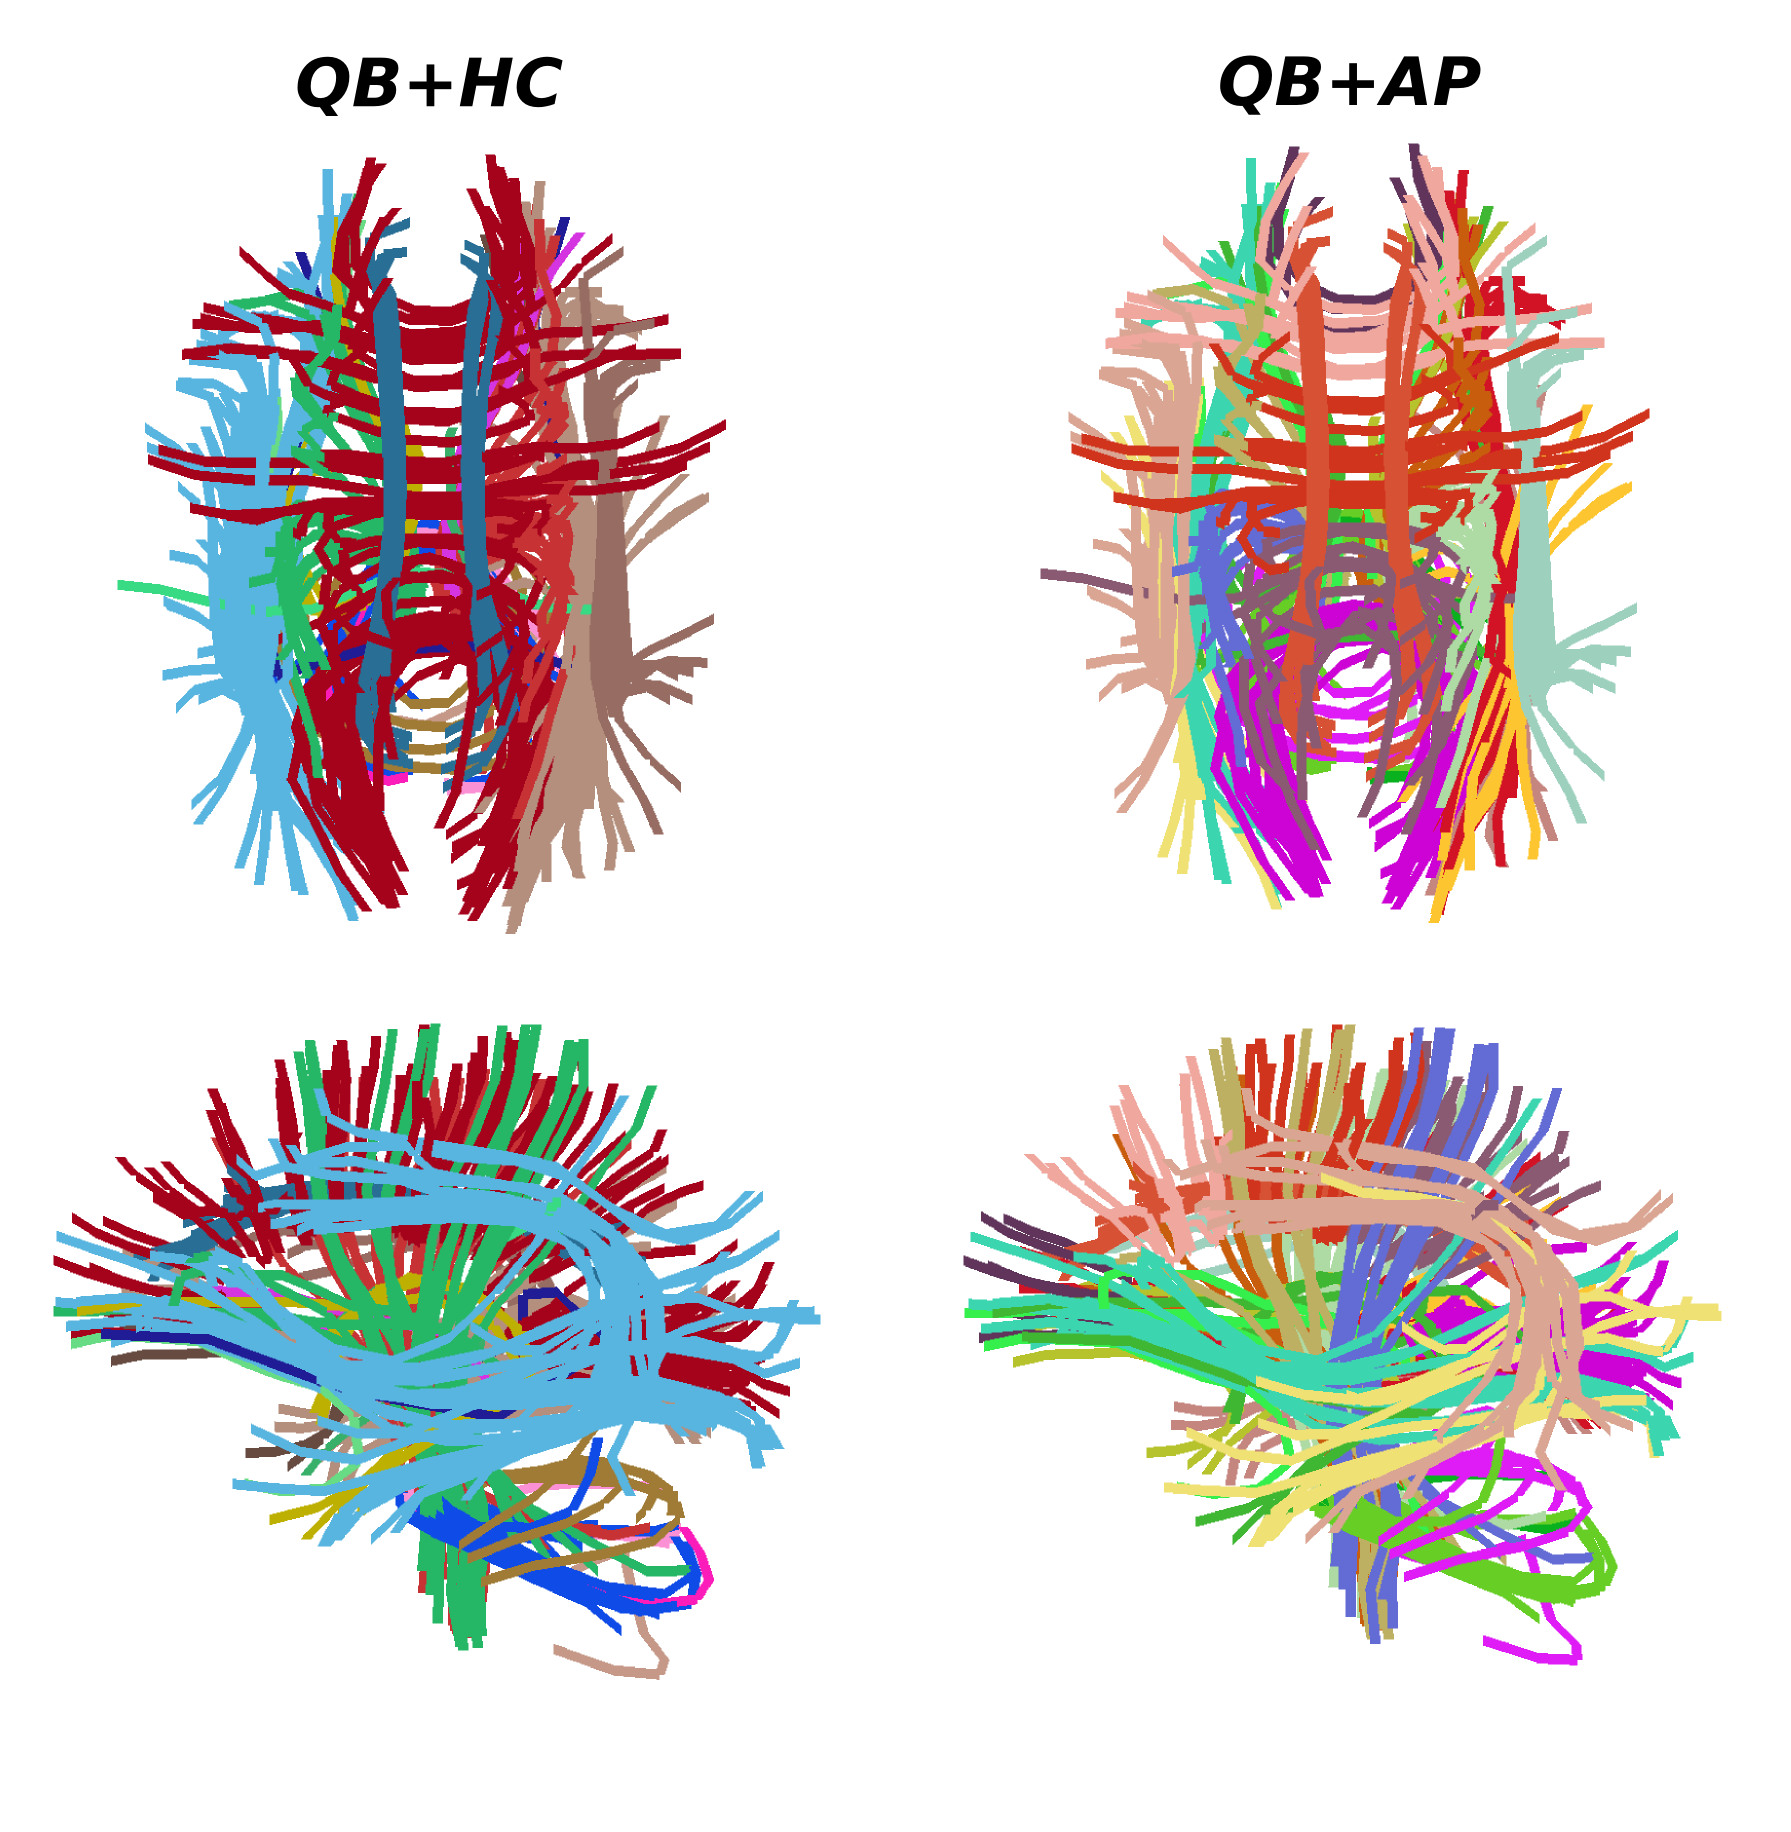
\includegraphics[scale=0.7]{last_figures/LSC_with_others}
\par\end{centering}

\label{Flo:LSC+HC+AP}
\caption{Two examples where QB output is used to cluster an entire set
  of $10$ tractographies together and then the result is given as input
  to hierarchical clustering (HC) using single linkage on the left and
  to affinity propagation (AP) on the right. Colours encode cluster
  labels. On the left side we see $19$ clusters and on the right
  $23$. QB facilitates significantly the operation of the other two
  algorithms which would not be able to cluster the entire data sets on
  current computers. Pay attention at the top left panel where QB+HC
  have managed to cluster the entire CC as one bundle.}

\end{figure}

For hierarchical clustering parts we used the software hcluster and for
affinity propagation we used the library scikit-learn. They are both
implemented in Python.

\subsection{Exemplars vs ROIs vs Masks}

Medical practitioners and neuroanatomists often argue that when they use
multiple spherical or rectangular masks to select some bundles many
tracks are thrown away because they are small and the mask operations
cannot get hold of them. Our method provides a solution to this problem
as it can identify broken or smaller bundles inside other bigger bundles
which are otherwise very difficult or even sometimes impossible to
identify visually or with the use of masks. Our method attacks this
problem and suggests a very efficient and robust solution which sets the
limit for unsupervised clustering of tractographies and facilitates
tractography exploration and interpretation. The point here is that one
can now use exemplar tracks as access points into the full tractography
and with a single click on that exemplar track obtain the entire bundle.
Therefore a super-bundle can be created just with with a few clicks
based on a selection from exemplar tracks.

In order to create this system we implemented a 3D
visualization/interaction system for tractographies based on QB in
Python and OpenGL. This project is available online at fos.me.


\section{Affinity Propagation\label{sub:Affinity-Propagation}}

Affinity propagation (AP) is a very recent $O(N^{2})$ clustering method
invented by \cite{frey2007clustering}, \cite{dueck2009affinity} which is
inspired by loopy belief propagation \cite{pearl1988probabilistic} and
other recent innovations in graphical models and more specifically is an
instance of the max-sum algorithm in factor graphs. For the completeness
of this thesis and because AP is a relatively new algorithm we give a
short description of the AP in this section. AP is an exemplar based
clustering method where the center of a cluster is a real data point
(exemplar) as in k-medoids, and k-centres rather than an average virtual
point as in k-means. AP starts by simultaneously considering all data
points as potential exemplars. Every data point is a node in a network
and AP recursively transmits real-valued messages along the edges of the
network until a good set of exemplars and corresponding clusters
emerges.

%
\begin{figure}
\noindent \begin{centering}
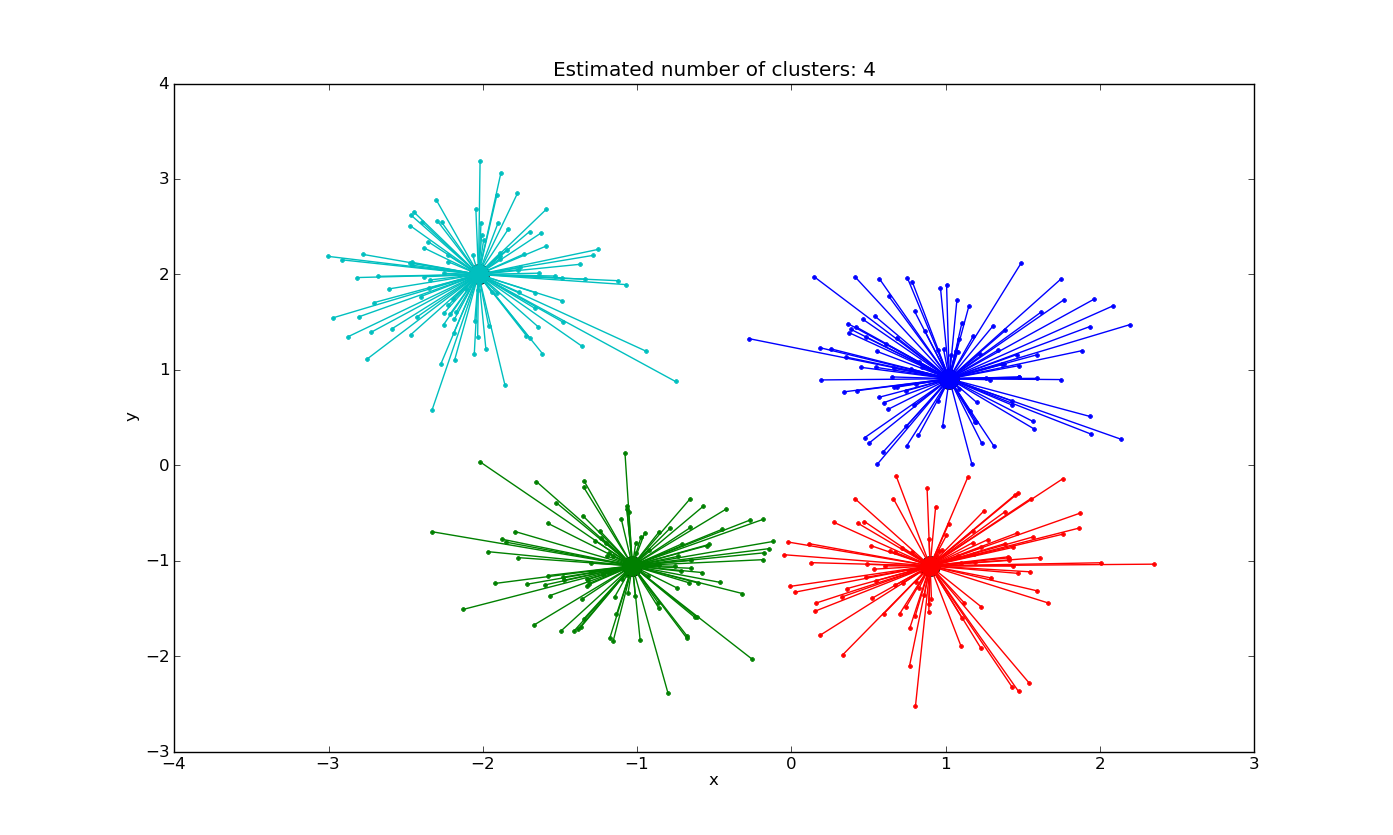
\includegraphics[scale=0.4]{last_figures/affinity_propagation_ok2}
\par\end{centering}

\label{Fig:AP_2d}

\caption{Simple example of affinity propagation at work where it can
  precisely identify 4 different normal distributions with means
  $(1,1),\;(-1,-1),\:(1,-1),$$(-2,2)$ and standard deviation $.5$. You
  can see the exemplars - most representative actual points - with
  thicker dots perfectly aligned with the means.}

\end{figure}

AP takes as input a collection of similarities between data points,
where the similarity $S(i,k)$ indicates how well the data point with
index $k$ is suited to be the exemplar for data point $i$. In order to
understand AP we can think just for the moment that we try to cluster 2D
data points and each similarity is expressed as the negative Euclidean
distance $S(i,k)=-||x_{i}-x_{k}||^{2}$ see Fig.\ref{Fig:AP_2d} therefore
$S$ for the moment is the negative complete squared distance matrix.
Rather than requiring the number of clusters to be prespecified, AP adds
a real number (preference weights) to the diagonal elements of $S$, one
for each data point so that larger values of $S(k,k)$ are more likely to
become exemplars. For, simplicity we can choose the $median(S)$ as the
common preference weight for all points; in this way we don't enforce
any \emph{a priori} information for one point to be an exemplar any more
than any other point. For some applications this could be an appropriate
requirement. There are two different messages exchanged between points
(1) responsibilities $R(i,k)=S(i,k)-{\displaystyle \max_{k':k'\neq
    k}}[S(i,k')+A(i,k')]$ and (2) availabilities which are initially
$A(i,k)=0$ and then equal to:

\begin{equation}
\forall i,k:\: A(i,k)=\begin{cases}
{\displaystyle \sum_{i':i'\neq i}} & max[0,\: R(i',k)],\: for\:\: k=i\\
\min & \left[0,\: r(k,k)+{\displaystyle \sum\max_{i':i'\notin\{i,k\}}[0,r(i',k)]}\right],\: for\:\: k\neq i\end{cases}\end{equation}


A very interesting fact is the way we get the final exemplars using
AP. 

After the messages have converged, there are two ways you can identify
exemplars: 

1) For data point $i$, $if\:\: R(i,i)+A(i,i)>0$, then data point
$i$ is an exemplar 

2) For data point $i$, $if\:\: R(i,i)+A(i,i)>R(i,j)+A(i,j)$, for
all $i$ not equal to $j$, then data point $i$ is an exemplar. 

Therefore, the availabilities and responsibilities are added to identify
exemplars. For point $i$, the value of $k$ that maximizes $A(i,k)+R(i,k)$
either identifies $i$ as an exemplar if $k=i$, or identifies the
data point that is the exemplar for point $i$. The message passing
procedure is terminated either after a fixed number of iterations,
or after changes in the messages stay low, or local decisions stay
constant; also the messages are damped - combining previous with current
message - to avoid numerical oscillations. 

Of course when we need to calculate distances between many points
then the distance matrix becomes too big for the available memory.
In that case if we are lucky and the data sets are sparse then we
can use AP on sparse matrices but if the data sets are not sparse
as it is the case with tractographies then we need to reduce the dimensionality
of the data sets and this why QB can be very handy. The complete algorithm
for AP is given in Alg.\ref{alg:AP}.

%
\begin{algorithm}
\label{alg:AP}\textbf{Input} Similarity/affinity matrix $S$ where the diagonal elements of $S(k,k)$ indicate the a priori preference for $k$ to be chosen as an exemplar \\
\textbf{Output} Clustering $CAP=\{c_{o},...,c_{k},...,c_{|CAP|-1}\}$, where a cluster $c=\{I,\mathbf{e},N\}$\\
$\forall i,k:\: A(i,k)=R(i,k)=0$\\
$S=S+n$ \# remove degeneracies\\
$d=0.5$ \# set damping factor\\
last\_iter=$100$ \# last iteration \\
$\textbf{For}$ iter $\textbf{From}$ $1$ $\textbf{To}$ last\_iter $\textbf{Do}$ \\
\hspace*{2em} $R_{old}=R$\\
\hspace*{2em} $\forall i,k:\: R(i,k)=S(i,k)-max_{k':k'\neq k}[S(i,k')+A(i,k')]$ \\
\hspace*{2em} $R=(1-d)R+d*R_{old}$ \# dampen responsibilities \\
\hspace*{2em} $A_{old}=A$ \\
\hspace*{2em} \# update availabilities \\
\hspace*{2em} $\forall i,k:\: A(i,k)=\begin{cases} \sum_{i':i'\neq i} & max[0,\: R(i',k)],\: for\:\: k=i\\ \min & \left[0,\: 	R(k,k)+{\displaystyle \sum\max_{i':i'\notin\{i,k\}}[0,R(i',k)]}\right],\: for\:\: k\neq i\end{cases}$ \\
\hspace*{2em} $A=(1-d)A+dA_{old}$ \# dampen availabilities \\
$\forall i, I_{e}=argmax\: S(i,I_{d})$ \# find indices of exemplars \\
$I_{e}(I_{d})=1:size\: (I_{d})$ \\
$L=I_{d}(I_{e})$ \# assign labels \\
$C_{AP}=\{c_{0},...,c_{k},...,c_{|C_{AP}|-1}\}$ \# clustering output\\
\# where a cluster $c=\{I,\mathbf{e},N\}$ holds the AP exemplars $\mathbf{e}$,\\
\# the indices $I$ of the cluster elements and $N$ the number of elements \\
\caption{Affinity Propagation}


\end{algorithm}

\section{Direct Tractography Registration}

Direct tractography registration is a recently described problem with
only a small number of publications, and so far as we know there are no
publicly available solutions. By direct registration we mean that no
other information apart from the tractographies themselves is used to
guide the registration. This is in contrast to the previous sections
where we used FA registration mappings applied to tractographies (see
section \ref{sub:Atlases-made-easy}) which is also most commonly used in
the literature along with other Tensor based
methods~\cite{goh2006algebraic}.

The currently described methodologies on this subject are as follows.
Leemans et al.~\cite{leemans2006multiscale} uses the invariance of
curvature and torsion under rigid registration along with Procrustes
analysis to co-register together different tractographies. Mayer et
al.~used iterative closest point applied to register pre-selected
bundles (bundles of interest - BOI) \cite{mayer2008bundles},
\cite{mayerdirect} and extended it using probabilistic boosting tree
classifiers for bundle segmentation
in\cite{mayer2011supervised}. Durrleman et
al.~\cite{durrleman2010registration} reformulated the tracks as currents
and implemented a currents based registration. Zvitia et
al.~\cite{zvitia2008adaptive} \cite{Zvitia2010}, used adaptive mean
shift clustering to extract a number of representative
fi{}bre-modes. Each fibre mode was assigned to a multivariate Gaussian
distribution according to its population thereby leading to a Gaussian
Mixture model (GMM) representation for the entire set of fibres. The
registration between two fibre sets was treated as the alignment of two
GMMs and is performed by maximizing their correlation ratio. A further
refinement was added using RANSAC\cite{fischler1981random} to obtain all
$12$ affine parameters. Ziyan et al.\cite{ZiyanMICCAI07} developed a
nonlinear registration algorithm based on the log-Euclidean polyaffine
framework\cite{Arsigny2009}; however this is not a direct tractography
registration algorithm as they first create scalar volumes, therefore
they do not try to register the tracks themselves in their space.

We now describe our algorithm and show that it is efficient and simple
to use, completely automatic and provides an evidently robust direct
rigid tractography registration algorithm available in seconds. This
algorithm could be of great use when comparing healthy versus severely
diseased brains e.g. stroke or vegetative state patients when non-rigid
registration is not recommended because of severe asymmetries in the
diseased brains. The algorithm is based on the robustness of QB to find
good representative descriptors.

\textbf{Procedure}. Here we describe a simple algorithm where $2$
tractographies $T_{A}$,$T_{B}$ are brought into alignment in native
space.
\begin{enumerate}
\item All tracks with length smaller than $100$mm and longer than $300$mm
are removed from the data sets. This will reduce the size of tractography
to about $1/4$ of its initial size ($~200,000$ tracks). (While all
the subjects are adults, this filtering may have different effects
depending on brain size. We have not investigated this question at
present.)
\item Both tractographies are equidistantly downsampled so every track contains
only $12$ points. 
\item We run QB with distance threshold at $10$mm for both tractographies.
\item Collect all exemplar tracks from clusters containing more than $0.2\%$
tracks. Let us assume we have these now in $E_{A}$ and $E_{B}$.
\item Calculate all pairwise distances $D=\mathtt{MDF}(E_{A},E_{B})$ and
save them in rectangular matrix $D$. 
\item Create a cost function (optimizer) which we will try to minimize the
symmetric minimum distance $\mathrm{SMD}=\sum_{i}\min_{j}D(i,j)+\sum_{j}\min_{i}D(i,j)$
.
\item Use modified Powell's method \cite{fletcher1987practical} to minimize
$\mathrm{SMD}$ over rigid rotations of $E_{\mathcal{B}}$ starting
with zeroed initial conditions. At each iteration of the optimization,
$E_{B}$ will be transformed by a rigid rotation and $\mathrm{SMD}$
will be recalculated. To ensure smooth rotations we use the Rodriguez
rotation formula.
\end{enumerate}
In Fig.\ref{Flo:direct_registration} A we see the result of this
algorithm applied to two tractographies -- represented with their
exemplar tracks -- depicted with orange and purple. We can see in the
upper panel that the orange tractography is misaligned with respect to
the purple one, and in the lower panel we see their improved alignment
after applying our algorithm.

\textbf{Metric}. SMD is proposed here for registration of trajectory
data sets, but one could equally use mutual
information\cite{maes1997multimodality} or the correlation ratio
\cite{roche1998correlation} for registration of volumetric data
sets. Nonetheless, the advantage of SMD is that it comes from robust
landmarks generated by QB which bring together local and global
components. Initially, it was not clear if we should use SMD or just the
sum of all distances $\mathrm{SD}=\sum_{i,j}D(i,j)$.  Therefore, we made
a small experiment to validate the smoothness and convexity of these two
cost functions. We plotted both functions under a single-axis
translation or a single-angle rotation of the same tractography as show
in Fig.\ref{Flo:direct_registration} B and C. From, these two diagrams
we can see that although for translations only the SD was entirely
convex, with rotations the SD had stronger local minima which is not a
good property for registration. Furthermore, the SMD had steeper
gradients towards the global minimum which is a positive indicator for
faster convergence.

\textbf{Experiments}. The first large scale experiment took place using
the same tractography of a single individual copied and transformed
$1000$ times with range of all three angles from $-45$ degrees to $45$
and range of all x,y,z translations from $-113$ to $113$mm.  Then we
registered all transformed tractographies to the static one and
calculated all pairwise MDF distances storing them in a square matrix
$D$. We would expect that if the registration was correct then the sum
of all diagonals elements of $D$ would be close to $0$.  This was
confirmed with both cost functions used SD and SMD getting close to zero
$99.8\%$ of the time however SMD was always closer to perfect alignment
than SD, having precision of more than $7$ decimals.  Consequently we
chosed SMD as a better cost function for direct tractography
registration.

We used GQI-based tractographies from $10$ subjects and we registered
all combinations of pairs $\binom{10}{2}=45$. Comparing different
tractographies is not a trivial problem however we can use the tightness
comparison (TC) metric explained in section
\ref{sub:Tightness-comparisons-1}.  We are happy to report the mean
initial TC was $34.8\%\pm8.0\%$ and the mean final TC after applying our
direct registration method was $48.1\%\pm6.1\%$. This was a
statistically highly significant improvement
($t_{\text{\textrm{paired}}}(44)=11.2$ ,$p\leq10^{-13}$ ). We are
planning in the future to compare this registration method against other
standard methods which are common in the literature.

%
\begin{figure}
\begin{centering}
\label{Flo:direct_registration}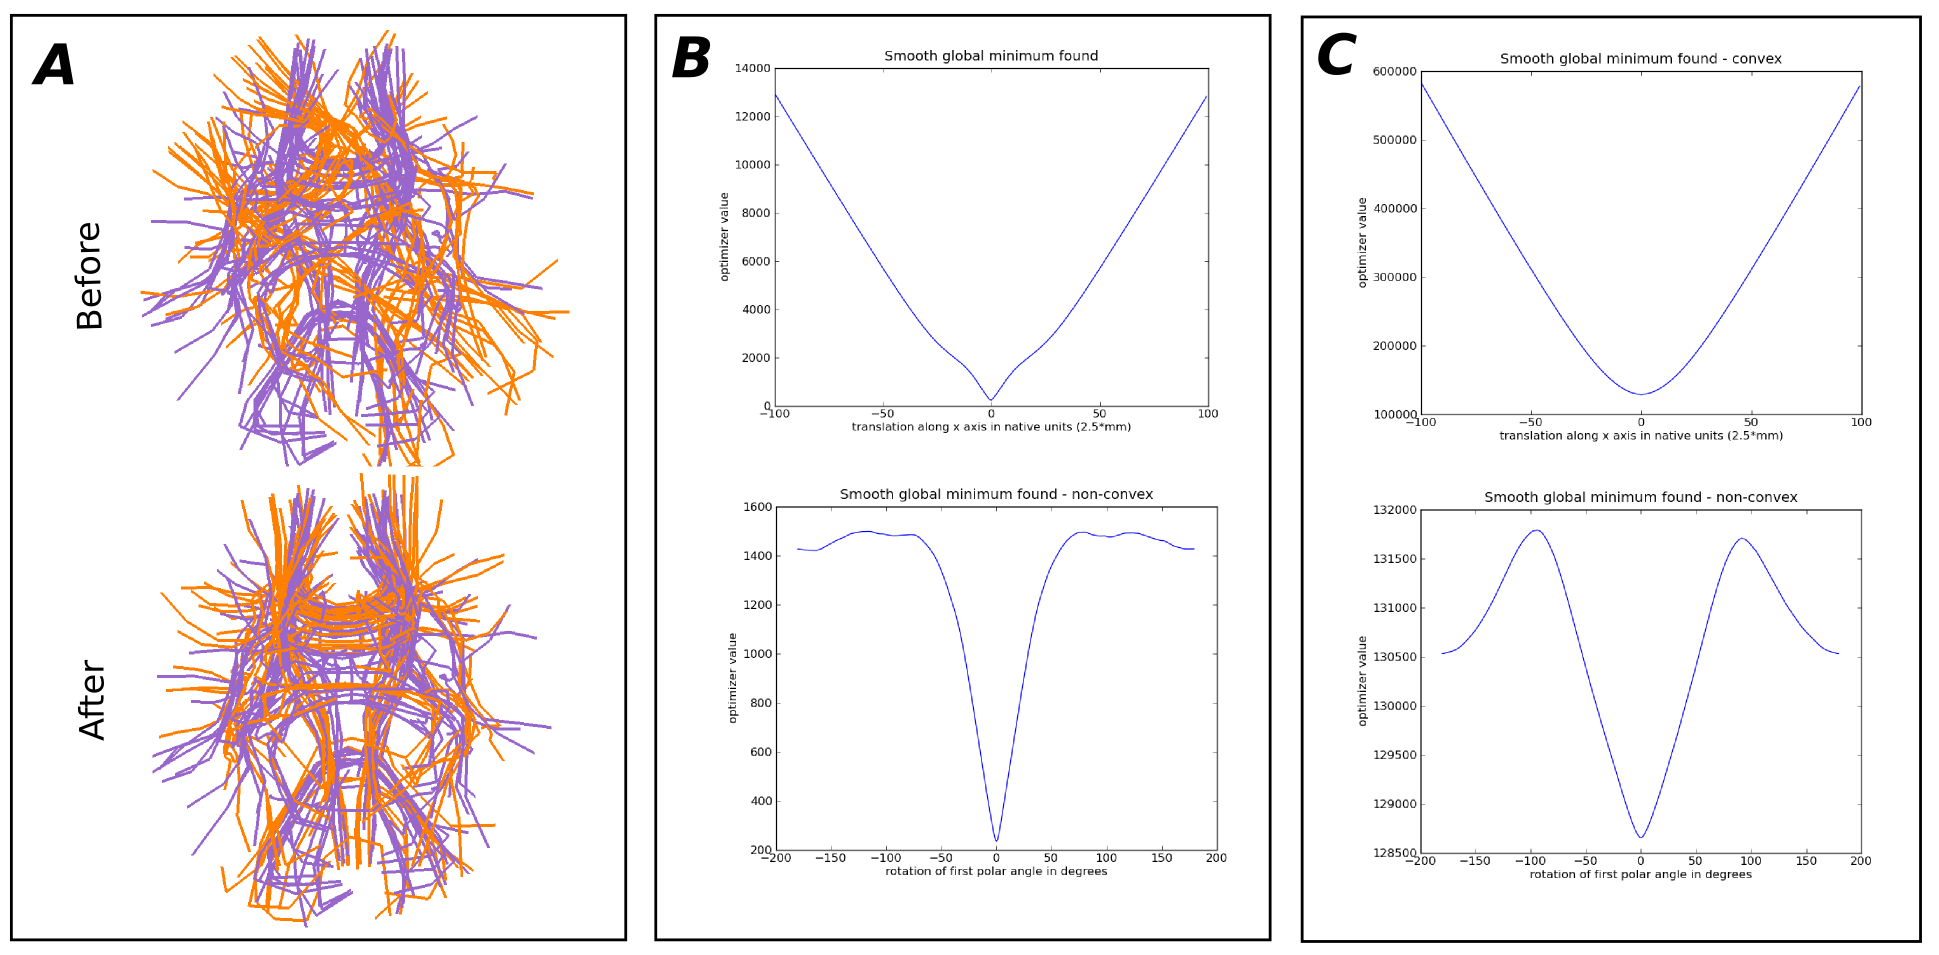
\includegraphics[scale=0.8]{last_figures/LSC_registration2}
\par\end{centering}

\caption{In panel A we see two tractographies from different subjects
  before (top) and after rigid registration (bottom) using our
  method. In panel B we see the metric $SMD$ that we chose to optimize
  for two copies of the same tractography with the second copy
  translated (above) and rotated (below). This metric appears to be
  smooth with a single global minimum and is only slightly non-convex
  with small local minima. In panel C another possible candidate metric
  $SD$ is shown which although more convex on translations it was much
  more problematic with rotations.}

\end{figure}

\section{Strategies with Small fibres}

In many parts of this document we did not consider short tracks. That
is perfectly valid because (a) the longer tracks are more likely to
be used as useful landmarks when comparing or registering different
subjects because it is more likely for them to exist in most subjects,
(b) removing short tracks facilitates the usage of distance based
clustering (no need for manually setting the distance threshold) and
interaction with the tractography, (c) someone would first want to
see the overall representation of the tractography and later go to
the details. Nonetheless, after having clustered the longer tracks
there are many ways to assign the smaller bundles to their closest
longer bundles. For this purpose we recommend to use a different distance
from $d_{df}$ (MDF) for example the minimum version of MAM referred
to as $\textrm{MAM}_{\textrm{min}}$ in Eq. [reference needed]
. 

%
\begin{figure}
\begin{centering}
\label{Flo:arcuate_close}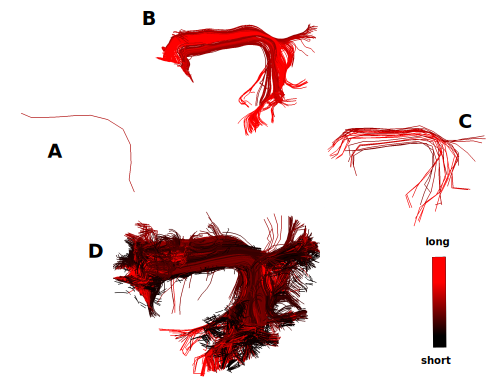
\includegraphics[scale=0.7]{last_figures/arcuate_small_fibers}
\par\end{centering}

\caption{A simple and vigorous strategy for handling short and long
  tracks together by picking a track of interest from one of our
  atlases. Colourmap here encodes track length. A: one picked selected
  atlas track, B: $245$ subject tracks closer than $15$mm (MDF
  distance), C: B tracks clustered in $23$ skeletons, D: $3421$ tracks
  closer than $6$mm (MAM distance) from the skeletons of B are shown. We
  can see that a great number of short tracks have been brought together
  along with the tracks in B. In that way we managed to bring together
  an entire bundle consisting both of long and short fibers by just
  selecting one track.}

\end{figure}


Here are some simple strategies for clustering short fibres. The first
is for unsupervised clustering and the second one is for supervised
learning.

\textbf{Strategy 1}. Cluster the long tracks using QB with distance
threshold at $10$mm and then cluster the short tracks (<$100$mm) to a
lower threshold and assign them to their closest long track bundle from
the first clustering using the $MAM_{min}$ distance.

\textbf{Strategy 2}. Read the tractography of a single subject, use a
tractographic atlas as the one created in section
\ref{sub:Atlases-made-easy} and pick one or more close skeletal tracks
from that atlas and then find the closest tracks from the subject to
that selected track using $d_{df}$, cluster the closest tracks found
from the previous step and for each one of these new skeletons find the
closest tracks using the $m_{in}$. We should now have an amalgamation of
shorter and longer fibres in one cluster.

An example of this second strategy is shown in
Fig. \ref{Flo:arcuate_close}: (A) a track of interest from the arcuate
fasciculus is selected from the tractographic atlas shown in
Fig. \ref{Flo:CloseToSelected}(top row-middle), (B) the tracks of the
subject closer than 15mm ($d_{df}$) from the selected cluster are shown
and clustered with a distance threshold of $6.25$mm in (C), (D) from
every skeleton track in C we find the closest tracks using the
($m_{in}$) distance from the entire tractography.


\section{Discussion and conclusion}

In this document we presented a novel and powerful algorithm --
QuickBundles (QB). This algorithm provides simplifications to the old
problem of white matter anatomy packing which has recently attracted
much scientific attention; it can also be used for any trajectory
clustering problem and it is recommended when large data sets are
involved. QB can be used with all types of diffusion MRI tractographies
which generate streamlines (e.g. probabilistic or deterministic) and it
is independent of the reconstruction model.

In common with mainstream clustering algorithms such as k-means,
k-centers and expectation maximization, QB is not a global clustering
method therefore it can give different results under different initial
conditions of the data set when there is no obvious distance threshold
which can separate the clusters in to meaningful bundles; for example we
should expect different clusters under different permutations/orderings
of the tracks in a densely packed tractography. However, we found that
there is enough agreement even between two clusterings of the same
tractography with different orderings. If the clusters are truly
separable by distances then there is a global solution independent of
orderings. This is often perceivable in smaller subsets of the initial
tractography. We empirically found that this problem is minimized even
with real data sets when a low distance threshold of about $10-20$ mm is
used.

Furthermore the output of QB can become now input for another recent
quick algorithm of quadratic time on average $O(M^{2})$ called affinity
propagation where now $M\ll N$ therefore the overall time stays linear
on the number of tracks $N$. Other algorithms previously too slow to be
used on the entire tractography can now be used efficiently too
e.g. kNN, hierarchical clustering and many others.

We saw that QB is a linear time clustering method based on track
distances, which is on average linear time $O(N)$ where $N$ is the
number of tracks and with worst case $O(N^{2})$ when every track is a
singleton cluster itself. Therefore QB is the fastest known tractography
clustering method and even real-time on tractographies with less than
$20,000$ tracks (depending on system CPU). We also showed that is uses a
negligible amount of memory.

QB is fully automatic and very robust as when we use it we can find good
agreements even between different subjects and can be used to create
tractography atlases at high speed. Additionally, it can be used to
explore multiple tractographies and find correspondences between
tractographies, create landmarks used for registration or population
comparisons.

QB can be used as well for reducing the dimensionality of the data sets
at the time of interaction; providing an alternative way to ROIs using
BOIs (bundles of interest) or TOIs (tracks of interest). We also showed
that it can be used to find {}``hidden'' tracks not visible to the user
at first instance. Therefore QB opens up the road to create a rapid
tools for exploring tractographies of any size.

The main concept of this clustering method is that a cluster can be
represented by virtual tracks which are used only during cluster
comparisons and not updated at every iteration.

A virtual (centroid) track is the average of all tracks in the cluster.
We call it virtual because it doesn't really exist in the real data set
and to distinguish it from exemplar (medoid) tracks which are again
descriptors of the cluster but are represented by real tracks.

The clustering creates a book of bundles/clusters which have easily
obtainable descriptors. When clusters are held in a tree structure this
permits upwards amalgamations to form bundles out of clusters, and
downwards disaggregation to split clusters into finer sub-clusters
corresponding to a lower distance threshold. However, we did not touch
this hierarchical extension of this algorithm here and mostly
concentrate on one level amalgamations.

We worked mostly with long tracks but strategies for short tracks
or bundles are straightforward and documented. We also showed an efficient
method where QB can speedup finding erroneous bundles or detecting
structures of specific characteristics.

We showed results with simulated, single or multiple real subjects
and the code for QuickBundles is freely available at dipy.org.

\section{References}

\selectlanguage{british}%
\bibliographystyle{elsarticle-harv}
\bibliography{diffusion}
\selectlanguage{english}

\end{document}
